%% -*- coding:utf-8 -*-
%%%%%%%%%%%%%%%%%%%%%%%%%%%%%%%%%%%%%%%%%%%%%%%%%%%%%%%%%
%%   $RCSfile: 5-hpsg-semantik.tex,v $
%%  $Revision: 1.22 $
%%      $Date: 2008/09/30 09:14:41 $
%%     Author: Stefan Mueller (CL Uni-Bremen)
%%    Purpose: 
%%   Language: LaTeX
%%%%%%%%%%%%%%%%%%%%%%%%%%%%%%%%%%%%%%%%%%%%%%%%%%%%%%%%%

\chapter{Semantik}
\label{chap-sem}\label{Kapitel-Semantik}


Innerhalb\is{Semantik|(} der HPSG"=Forschung gibt es drei verschiedene Ansätze
zur Beschreibung der Bedeutung sprachlicher Ausdrücke. In den ersten
HPSG"=Arbeiten \citep{ps,ps2,Kiss95a,Mueller99a} und auch in einigen Umsetzungen 
innerhalb der Computerlinguistik \citep{MuellerBabel} wurde die Situationssemantik
\citep*{BP83a,CMP90,Devlin92}\nocite{BP87a} verwendet. Ab den frühen 1990ern gab es Arbeiten zur Unterspezifikationssemantik
\citep{Nerbonne93a}. Zu dieser Art Semantik zählen die \emph{Lexical Resource Semantics} (LRS,
\citealt{RS2004a-u,IR2015a-u,Richter2016a-u,SailerRichter2021a-u}, \citealt[Section~6.2]{KR2024a}), die \emph{Minimal Recursion Semantics}\is{Minimal Recursion Semantics@\emph{Minimal Recursion Semantics} (MRS)}
(MRS, \citealt*{CFPS2005a}) und Varianten der \emph{Discourse Representation Theory} (DRT, \citealt{KR93a}) mit Underspecified
Discourse Representation Structures (UDRS, \citealt{FR95a-u}). Zur MRS gab es 1995 die ersten Veröffentlichungen \citep{CFMRS95a-u} und
der 2005er Aufsatz kursierte
in verschiedenen Versionen seit dieser Zeit im Netz. Veröffentlichungen wie das Buch von
\citet{GSag2000a-u}, das Situationssemantik verwendet, kamen nur noch selten vor. Auch UDRS haben
sich nicht wirklich durchgesetzt. Das Buch von \citet{Holler2005a-u} blieb eine Ausnahme.
Während die LRS hauptsächlich in Frankfurt/Main verwendet wird, ist MRS
weiter verbreitet. MRS wird in theoretischen Arbeiten (\zb \citealt{Kiss2001a}) benutzt, aber auch in
Computerimplementationen und Übersetzungssystemen \citep*{FCS2000a,MK2000a,Siegel2000a,BFO2002a-u,MuellerCoreGram}. MRS ist für computerlinguistische Systeme gut geeignet, da
Skopusbeziehungen\is{Skopus} unterspezifiziert dargestellt werden können, was eine effizientere
Verarbeitung der Grammatiken durch Computer ermöglicht. Zu weiteren Vorteilen siehe \citep*[Abschnitt~2]{CFPS2005a}.
Das folgende Kapitel führt in MRS ein. Dazu diskutiere ich viele der Anwendungsfälle, die für das
Englische von \citet*{CFPS2005a} ausgearbeitet wurden. Für Details, die in diesem klassischen Papier
offen geblieben sind, habe ich die implementierte Grammatik von Dan Flickinger konsultiert
\parencites{Flickinger2000a,FCS2000a}. Die ersten drei Auf"|lagen dieses Buches haben noch
Situationssemantik verwendet. Leser*innen, die die Ansätze vergleichen möchten, können also frühere
Auflagen konsultieren.

Dieses Buch ist ein Syntax"=Buch. Syntax ist ein komplexes System und die Beschäftigung damit
faszinierend. Allerdings ist Syntax allein im wahrsten Sinne des Wortes sinnlos. Die (Morpho-)Syntax wird nur gebraucht, um eine
Verbindung zwischen der lautlichen Form einer Äußerung und ihrer Bedeutung herzustellen: Eine
Hörer*in ist nur in der Lage herauszufinden, was eine Sprecher*in mit ihrer Äußerung meint, wenn
sie in der Lage ist, die Laute in Wörter und Wortgruppen zu strukturieren und einzelnen Wörtern,
größeren Einheiten und schließlich dem gesamten komplexen Gebilde
eine Bedeutung zuzuordnen, \dash aus der Bedeutung einzelner Wörter, die Bedeutung der gesamten
Äußerung zu ermitteln. Wenn es die Aufgabe der Syntax ist, entsprechende Strukturen bereitzustellen,
muss man als Grammatiker*in auch sagen können, wie Bedeutung repräsentiert wird und wie die
Bedeutungskomposition mittels syntaktischer Strukturen funktioniert. In jedem Grammatikframework
muss es dazu Überlegungen geben. Verglichen mit anderen Theorien wird bei vielen HPSG"=Arbeiten
neben der Syntax auch über die Semantik eines bestimmten Phänomens gesprochen.

Im Gegensatz zu Ausdrücken in Programmiersprachen sind natürlichsprachliche Ausdrücke oft
mehrdeutig. Leider gibt es Mehrdeutigkeiten auf den verschiedensten sprachlichen Ebenen. Schon bei der Gruppierung der
Lautfolgen eines akustischen Signals in Wörter gibt es oft sehr viele
Möglichkeiten. Unter Wissenschaftler*innen, die in der Spracherkennung arbeiten, wird der folgende
Satz gern als Beispiel benutzt:
\ea
It is easy to wreck a nice beach.
\z
Wenn man diesen Satz äußert, nachdem man über speech recognition (Erkennung gesprochener Sprache)
gesprochen hat, werden alle \emph{It is easy to recognize speech.} verstehen. Außerdem gibt es
Ambiguitäten bei den Wortbedeutungen (\emph{der Kiefer} vs.\ \emph{die Kiefer}) und es gibt oft
mehrere mögliche syntaktische Strukturen oder auch verschiedene Interpretationen von Quantoren wie
\emph{alle}, \emph{jeder} und \emph{ein}. Das alles ist für kompetente Sprecher*innen einer Sprache
kein Problem. Nicht-Linguist*innen nehmen die Ambiguitäten normalerweise nicht wahr, weil unsere
Gehirne Kontextwissen einbeziehen und weil Strände eben irrelevant sind, wenn es gerade um
Spracherkennung geht. %Die Ausnahmen kann man dann im Hohlspiegel bewundern.
(\mex{1}) zeigt einige Beispiele aus den Bereichen, die uns hier interessieren:
\eal
\ex Unbekannte haben Mittwochabend bei einer %FDP-Wahlkampfveranstaltung\\
FDP-Wahlkampfveranstaltung mit FDP-Chef Guido Westerwelle Farbbeutel geworfen.\footnote{
taz, 21.5.2004, S.\,7
}
\ex
\label{ex-Jede-Tochter-eines-Mitarbeiters-schläft}
Jede Tochter eines Mitarbeiters schläft.
\zl 
(\mex{0}a) hat zwei Lesarten: In der ersten findet eine Wahlkampfveranstaltung mit dem FDP-Chef
statt und bei der zweiten wirft Guido Westerwelle gemeinsam mit Unbekannten Farbbeutel. Die
Mehrdeutigkeit entsteht dadurch, dass es zwei verschiedene syntaktische Strukturen gibt. In der einen ist
\emph{mit FDP-Chef Guido Westerwelle} Bestandteil der NP \emph{einer FDP"=Wahlkampfveranstaltung mit
  FDP-Chef Guido Westerwelle} und in der anderen modifiziert die \emph{mit}"=PP \emph{geworfen}.
Es ist die Aufgabe der Syntax die Mehrdeutigkeit des Satzes zu erklären. Interessanter für die
Diskussion in diesem Kapitel ist der Satz in (\mex{0}b). Hier entspricht \emph{jede} dem Allquantor ($\forall$) und \emph{eine} dem
Existenzquantor ($\exists$), der vielleicht schon aus der Mathematik bekannt ist.\footnote{%
Für eine Einführung in die Logik für Sprachwissenschaftler*innen siehe \citew*{AAD73a} oder \citew{Lohnstein2011a}.}
Es gibt dann zwei Lesarten: In der einen muss es einen bestimmten Mitarbeiter geben
und für alle Töchter, die er hat, muss gelten, dass sie schlafen. Man sagt, dass der Existenzquantor
\isi{Skopus} über den Allquantor hat. In der anderen Lesart muss für alle
Menschen, für die gilt, dass sie die Tochter eines Mitarbeiters sind, gelten, dass sie
schlafen. Hier sagt man der Allquantor hat Skopus über den Existenzquantor. Denkt man nun über die
Struktur von (\ref{ex-Jede-Tochter-eines-Mitarbeiters-schläft}) nach, so wird klar, dass man eigentlich eine eindeutige syntaktische
Struktur haben möchte. Die Struktur für die NP \emph{jede Tochter eines Mitarbeiters} haben wir
bereits in Abbildung~\ref{fig-die-Tochter-eines-Mitarbeiters} auf
S.\,\pageref{fig-die-Tochter-eines-Mitarbeiters} gesehen und auch bei der Kombination mit
\emph{schläft} entstehen keine Mehrdeutigkeiten. Es gibt aber in der Tat Ansätze, die
von syntaktischen Mehrdeutigkeiten ausgehen. Zum Beispiel haben \citet{Chomsky76a-u} und
\citet{May77a-u,May85a-u} im Rahmen der Transformationsgrammatik \citep{Chomsky57a,Chomsky81a} vorgeschlagen, dass die verschiedenen Lesarten durch das Bewegen der Quantoren in
syntaktischen Strukturen (auf der so genannten Logischen Form\is{Logische Form}) entstehen. Frühere HPSG"=Ansätze
verwenden Speicher für Quantoren und man kann die Quantoren dann an unterschiedlichen Stellen in
syntaktischen Strukturen aus dem Speicher entnehmen \parencites{Cooper83}[Kapitel~8]{ps2}. Da in der
HPSG syntaktische und semantische Aspekte in einer gemeinsamen Struktur behandelt werden, bekommt
man dann aber auch für Sätze wie (\ref{ex-Jede-Tochter-eines-Mitarbeiters-schläft}) zwei verschiedene Strukturen. Man kann sich klar machen, dass sich strukturelle
Mehrdeutigkeiten multiplizieren. Mehrdeutigkeiten in Nominalphrasen multiplizieren sich mit
Mehrdeutigkeiten wie denen, die in (\mex{0}a) vorliegen. Auch ist es so, dass es bei gleichzeitigem
Vorliegen mehrerer Quantoren in verschiedenen NPen im Satz unglaublich viele Lesarten geben kann, die
letztendlich nur Expert*innen anhand sorgfältig konstruierter Kontexte unterscheiden können. Wenn
man also eine Semantikrepräsentation hat, die genau die Skopusbeziehungen unterspezifiziert lässt, dann kann
man, so wie das Menschen tun \citep{FBF2002a-u,Dwivedi2013a-u,Frances2024a-u}, 
die Bedeutung komprimiert verpackt lassen und sie erst dann
auflösen, wenn man genug Evidenz dafür hat, welche Lesart vom Sprecher beabsichtigt war.
Im Folgenden werden wir uns mit MRS beschäftigen, einem Semantikformalismus, der genau das möglich
macht: eine unterspezifizierte Semantikrepräsentation für (\ref{ex-Jede-Tochter-eines-Mitarbeiters-schläft}), in der die zwei Lesarten
enthalten sind.

Das Kapitel ist wie folgt strukturiert: In Abschnitt~\ref{sec-Relationen-und-Merkmalbeschreibungen}
zeige ich, wie man die Bedeutung von Nomen und Verben erfasst und wie man die entsprechenden
Relationen mit Merkmalbeschreibungen darstellen kann. Abschnitt~\ref{sec-CONT} erklärt, wie die
Bedeutung in sprachlichen Zeichen repräsentiert wird und warum die Merkmalsgeometrie so angepasst
wird, dass alle syntaktisch relevanten Merkmale gemeinsam in einer Teilstruktur repräsentiert
werden. Abschnitt~\ref{sec-index} beschäftigt sich mit dem semantischen Beitrag nominaler Objekte
und Abschnitt~\ref{sec-Linking}
zeigt, wie man die Verbindung zwischen den Argumenten eines Kopfes und dem semantischen Beitrag des
Kopfes herstellen kann, \dash, es wird gezeigt, wie die semantischen Rollen einer Relation gefüllt
werden können. Abschnitt~\ref{sec-Komposition} erklärt, wie einfache kompositionale Semantik
funktioniert und Abschnitt~\ref{sec-Skopus} schließlich beschäftigt sich mit Quantorenskopus und
diversen interessanten Phänomenen, die für das Verständnis des technischen Apparats notwendig sind.




\section{Relationen und ihre Repräsentation in Merkmalbeschreibungen}
\label{sec-Relationen-und-Merkmalbeschreibungen}

Über die Bedeutung von Wörtern kann man lange nachdenken: Was bedeutet es, jemanden oder etwas zu
lieben? Was bedeutet das Wort \emph{Tasse}? Muss das Objekt, auf das wir uns beziehen eine bestimmte
Form haben? Einen Henkel? Warum ist ein Eimer etwas Anderes als eine Tasse? Was macht eine Zitrone
aus? Dass sie gelb ist und sauer? Ist eine grüne Zitrone keine Zitrone \citep{Braisby90}? All das sind spannende
Fragen, mit denen sich Semantiker*innen auch beschäftigen \citep{Rosch1973b-u}. Hier spielen sie aber keine Rolle, denn
man kann sich damit behelfen, dass man dem Bündel an Eigenschaften einfach einen Namen gibt: Für die Bedeutung von \emph{lieben} verwendet man die
Relation \relation{lieben} und für die von \emph{Zitrone} die Relation \relation{zitrone}. Man muss
dann immer noch klären, wofür \relation{zitrone} genau steht, aber für die Interaktion mit der
Syntax ist die Repräsentation über Relationen mit Argumenten ausreichend. Die Bezeichnungen für die
Relationen sind willkürlich gewählt. Für das Deutsche nimmt man die Nennform. Das ist bei Verben der
Infinitiv ohne \emph{zu} und bei Nomen die Nominativ"=Singular"=Form. Dass es sinnvoll ist, von der
Flexionsform von Wörtern zu abstrahieren zeigen die folgenden Sätze:
\eal
\label{ex-Alle-Delfine}
\ex Jeder Delfin liebt ein Känguru.
\ex Alle Delfine lieben ein Känguru.
\zl
Die Frage, ob \emph{Delfin} im Satz im Singular oder Plural steht und wie die Form von \emph{lieben}
aussieht, ist für die Bedeutung letztendlich irrelevant. Deshalb ist es sinnvoll, sich für die
Bedeutungsrepräsentation auf eine Form der entsprechenden Wörter zu einigen.

Relationen können verschiedene Stelligkeiten haben. Je nach Ansatz werden Relationen wie
\relation{lieben} als zweistellig oder dreistellig eingestuft. Geht man von einem zweistelligen
\relation{lieben} aus, dann sind nur der bzw.\ die Liebende und der/die/das Geliebte Argumente der
\relation{lieben}"=Relation. Die Alternative ist, dass man annimmt, dass ein lieben"=Ereignis
beschrieben wird und das Ereignis in Relation zu Liebendem und Geliebtem steht. Ich gehe hier von
Letzterem aus. Somit ergeben sich die folgenden Stelligkeiten:
\begin{itemize}
\item einstellig:  \relation{regnen}   (\emph{Es regnet.}) 
\item zweistellig: \relation{sterben}  (\emph{Aicke stirbt.})
\item dreistellig: \relation{lieben}   (\emph{Aicke liebt Conny.})
\item vierstellig: \relation{geben}    (\emph{Aicke gibt Conny den Aufsatz.})
\item fünfstellig: \relation{kaufen}   (\emph{Aicke kauft den gebrauchten Mantel vom Conny für fünf Euro.})
\end{itemize}
Für die Bedeutungsrepräsentation wird von der konkreten Realisierung im Satz abstrahiert. 
In der Prädikatenlogik\is{Prädikatenlogik} wird \zb dem Satz (\mex{1}a) die Repräsentation (\mex{1}b) zugeordnet.
\eal
\ex Aicke liebt Conny.
\ex \relation{lieben}(e, Aicke$'$, Conny$'$)
\zl
Das kleine $e$ steht dabei für das Ereignis. Das $e$ wird auch Ereignisvariable
genannt. \relation{Aicke} und \relation{Conny} sind sogenannte Individuenkonstanten. Dieselbe Bedeutung kann aber auch durch den Passivsatz in (\mex{1}) ausgedrückt werden.
\ea
Conny wird von Aicke geliebt.
\z
Eigennamen und Nomina referieren auf Personen (\emph{Aicke}, \emph{Conny}, \emph{Tochter}), Objekte (\emph{Tasse},
\emph{Stuhl}, \emph{Fahrrad}) oder Konzepte (\emph{Angst}, \emph{Freude}). Man bezieht sich in der
Semantik oft auf ein Diskursuniversum. Das ist der Ausschnitt der Welt, über den gerade
gesprochen wird. Das ist sinnvoll, denn man kann in einer Wohnung den Satz \emph{Alle Kinder
  schlafen.} äußern und er ist für die relevante Situation wahr. Würde man jedoch den Wahrheitswert
in Bezug auf eine ganze Stadt oder die ganze Welt bestimmen wollen, so wäre der Satz wohl falsch,
denn ein Kind ist immer irgendwo wach.
In Diskursuniversen gibt es Individuen (Personen, Objekte, abstrakte Konzepte), auf
die man sich beziehen kann. \relation{tochter}(x, y) drückt aus, dass zwischen x und y die
\relation{tochter}"=Relation besteht, \dash, dass x die Tochter von y im betreffenden
Diskursuniversum ist. Mit \relation{fahrrad}(x) kann man ausdrücken, dass das Objekt x die
Eigenschaft hat, ein Fahrrad zu sein. Auch für Adjektive gibt es Relationen. Relationen lassen sich
mit logischen Operatoren verknüpfen: \relation{gelb}(x) $\wedge$ \relation{fahrrad}(x) steht für
etwas, das gelb und ein Fahrrad ist, also ein gelbes Fahrrad.

Abbildung~\ref{fig-Diskursuniversum-Konstanten} zeigt ein Diskursuniversum mit verschiedenen
Individuen. Diesen sind Bezeichner, die Individuenkonstanten, zugeordnet. Ein Individuum kann einen,
zwei oder auch gar keinen Bezeichner haben. Das arme Individuum rechts oben in der Abbildung hat
keinen Bezeichner. In normalen Diskursuniversen haben die meisten Individuen keine dazugehörige
Individuenkonstante. In einer Wohnung haben wir normalerweise Tische, Stühle, Schränke, ein Klo und
außer Ingo dem Esstisch, hat keines dieser Objekte einen Namen. In der
Abbildung~\ref{fig-Diskursuniversum-Konstanten} könnte es sich bei dem Objekt rechts oben um eine
Staubfluse handeln. Zu Staubflusen entwickeln die wenigsten Menschen eine so innige Beziehung, dass
sie ihr einen Namen geben.
\begin{figure}
	\begin{tikzpicture}[scale=0.75]
		\draw (0,0) rectangle (8,5);
		%
		\node[anchor=west] at (1.5,0.5) {Kirby};
		\node[anchor=west] at (2.3,1.7) {Aicke};
		\node[anchor=east] at (1.8,3) {sweety};
		\node[anchor=west] at (3.5,3.5) {Conny};
		%
		\draw (1,1) -- (1.6,0.7); %Kirby
		\draw (2,2) -- (2.4,1.9); %Aicke
		\draw (2,2) -- (1.4,2.7); %sweety
		\draw (3,3) -- (3.6,3.3); %Conny
		%
		\draw[fill=fugreen, draw=black] (1,1) circle (0.1);
		\draw[fill=fugreen, draw=black] (2,2) circle (0.1);
		\draw[fill=fugreen, draw=black] (3,3) circle (0.1);
		\draw[fill=fugreen, draw=black] (4,2) circle (0.1);
		\draw[fill=fugreen, draw=black] (7,4) circle (0.1);
	\end{tikzpicture}
% \begin{pspicture}(0,0)(8,5)
% %\psgrid
% \psframe(0,0)(8,5)
% \rput[Bl](2.6,1.2){%
% \rnode{Aicke}{Aicke}}
% \rput[Bl](1,3){%
% \rnode{sweety}{sweety}}
% \rput[Bl](4,3){%
% \rnode{Conny}{Conny}}
% \rput[Bl](2,.5){%
% \rnode{Kirby}{Kirby}}

% \cnode[fillcolor=fugreen,fillstyle=solid](1,1){0.1}{KirbyDot}
% \cnode[fillcolor=fugreen,fillstyle=solid](2,2){0.1}{AickeDot}
% \cnode[fillcolor=fugreen,fillstyle=solid](4,2){0.1}{NonameDot}
% \cnode[fillcolor=fugreen,fillstyle=solid](3,3){0.1}{ConnyDot}
% \cnode[fillcolor=fugreen,fillstyle=solid](7,4){0.1}{NoName2Dot}
% %
% %\psellipse(4,2)(3,1.5)
% %\anodeconnect[l]{modell}[r]{phen}%
% \ncline[nodesepA=2pt,nodesepB=0pt]{Kirby}{KirbyDot}
% \ncline[nodesepA=2pt,nodesepB=0pt]{Aicke}{AickeDot}
% \ncline[nodesepA=2pt,nodesepB=0pt]{sweety}{AickeDot}
% \ncline[nodesepA=2pt,nodesepB=0pt]{Conny}{ConnyDot}
% \end{pspicture}
\caption{Diskursuniversum mit Individuen, denen Individuenkonstanten zugeordnet sind}\label{fig-Diskursuniversum-Konstanten}
\end{figure}

Abbildung~\ref{fig-Diskursuniversum-blond} zeigt die Menge der blonden Individuen im Diskursuniversum.
\begin{figure}
	\begin{tikzpicture}[scale=0.75]
		\draw (0,0) rectangle (8,5);
		\draw (1.5,1.5) circle (1);
		\draw[fill=fugreen, draw=black] (1,1) circle (0.1);
		\draw[fill=fugreen, draw=black] (2,2) circle (0.1);
		\draw[fill=fugreen, draw=black] (3,3) circle (0.1);
		\draw[fill=fugreen, draw=black] (4,2) circle (0.1);
		\draw[fill=fugreen, draw=black] (7,4) circle (0.1);
		%
		\node[anchor=west] at (3,0.5) {blond};
		\draw (2.3,0.9) -- (3,0.7);
	\end{tikzpicture}
% \begin{pspicture}(0,0)(8,5)
% %\psgrid
% \psframe(0,0)(8,5)
% \pscircle[fillcolor=fugreen,fillstyle=solid](1,1){0.1}
% \pscircle[fillcolor=fugreen,fillstyle=solid](2,2){0.1}
% \pscircle[fillcolor=fugreen,fillstyle=solid](4,2){0.1}
% \pscircle[fillcolor=fugreen,fillstyle=solid](3,3){0.1}
% \pscircle[fillcolor=fugreen,fillstyle=solid](7,4){0.1}
% \rput[Bl](3,0.5){%
% \rnode{blond}{blond}}
% %
% \cnode(1.5,1.5){1}{blondSet}
% \ncline[nodesepA=0pt,nodesepB=2pt]{blondSet}{blond}
% \end{pspicture}
\caption{Diskursuniversum mit der Menge der blonden Individuen}\label{fig-Diskursuniversum-blond}
\end{figure}

Abbildung~\ref{fig-Diskursuniversum-blond-Kind} zeigt zwei Mengen: die der blonden Individuen und
die der Kinder. Mann kann hier schön sehen, dass die Schnittmenge dieser beiden Mengen genau der
Menge der blonden Kinder entspricht.
\begin{figure}
\nomemoize{
	\begin{tikzpicture}[scale=0.75]
		\draw (0,0) rectangle (8,5);
		% 
		\begin{scope}
			\clip (3,2) circle (1.5);
			\fill[pattern=north east lines] (1.5,1.5) circle (1);
		\end{scope}
		% 
		\draw (1.5,1.5) circle (1);
		\draw (3,2) circle (1.5);
		% 
		\draw[fill=fugreen, draw=black] (1,1) circle (0.1);
		\draw[fill=fugreen, draw=black] (2,2) circle (0.1);
		\draw[fill=fugreen, draw=black] (3,3) circle (0.1);
		\draw[fill=fugreen, draw=black] (4,2) circle (0.1);
		\draw[fill=fugreen, draw=black] (7,4) circle (0.1);
		% 
		\node[anchor=east] at (1.5,3.5) {blond};
		\draw (0.8,3.3) -- (1.1,2.4);
		% 
		\node[anchor=west] at (5,3) {Kind};
		\draw (4.1,3) -- (5,3);
	\end{tikzpicture}}
% \begin{pspicture}(0,0)(8,5)
% %\psgrid
% \psframe(0,0)(8,5)
% \rput[Bl](5,3){%
% \rnode{Kind}{Kind}}
% %
% \cnode(3,2){1.5}{KindSet}
% \ncline[nodesepA=0pt,nodesepB=2pt]{KindSet}{Kind}
% \rput[Bl](0.5,3.5){%
% \rnode{blond}{blond}}
% %
% \cnode(1.5,1.5){1}{blondSet}
% \ncline[nodesepA=0pt,nodesepB=2pt]{blondSet}{blond}
% \psclip
% {%
% \pscircle(3,2){1.5}
% }
% \pscircle[fillstyle=hlines](1.5,1.5){1}
% \endpsclip
% \pscircle[fillcolor=fugreen,fillstyle=solid](1,1){0.1}
% \pscircle[fillcolor=fugreen,fillstyle=solid](2,2){0.1}
% \pscircle[fillcolor=fugreen,fillstyle=solid](4,2){0.1}
% \pscircle[fillcolor=fugreen,fillstyle=solid](3,3){0.1}
% \pscircle[fillcolor=fugreen,fillstyle=solid](7,4){0.1}
% %
% %\psellipse(4,2)(3,1.5)
% %\anodeconnect[l]{modell}[r]{phen}%
% \end{pspicture}
\caption{Diskursuniversum mit Menge von blonden Individuen und von Individuen mit der Eigenschaft,
  Kind zu sein, und der Schnittmenge der blonden Kinder}\label{fig-Diskursuniversum-blond-Kind}
\end{figure}

Abbildung~\ref{fig-Diskursuniversum-blond-Kind-schlafen} zeigt zusätzlich noch die Menge der
schlafenden Individuen. Da die Menge aller blonden Kinder eine Teilmenge der schlafenden Individuen
ist, ist der Satz (\mex{1}a) im vorliegenden Diskursuniversum wahr.
\eal
\ex Alle blonden Kinder schlafen.
\ex Ein blondes Kind schläft.
\zl
Da es im Diskursuniversum ein blondes Kind gibt und dieses schläft, ist auch der Satz in (\mex{0}b) wahr.
\begin{figure}
\nomemoize{%
\begin{tikzpicture}[scale=0.75]
		\draw (0,0) rectangle (8,5);
		\draw (1.5,1.5) circle (1); %klug
		\draw (3,2) circle (1.5);  %Kind
		\draw[rotate around={50:(2.4,2.4)}] (2.5,2.5) ellipse (1.5 and 0.9); %schlafen 
		%
		\begin{scope}
			\clip (1.5,1.5) circle (1);
			\clip (3,2) circle (1.5);
			\clip[rotate around={50:(2.4,2.4)}] (2.5,2.5) ellipse (1.5 and 0.9);
			\fill[pattern=north east lines] (0,0) rectangle (8,5);
		\end{scope}
		%
		\draw[fill=fugreen, draw=black] (1,1) circle (0.1);
		\draw[fill=fugreen, draw=black] (2,2) circle (0.1);
		\draw[fill=fugreen, draw=black] (3,3) circle (0.1);
		\draw[fill=fugreen, draw=black] (4,2) circle (0.1);
		\draw[fill=fugreen, draw=black] (7,4) circle (0.1);
		%
		\node[anchor=east] at (1.5,3.5) {blond};
		\draw (0.8,3.3) -- (1.1,2.4);
		%
		\node[anchor=west] at (5,3) {Kind};
		\draw (4.1,3) -- (5,3);
		%
		\node[anchor=west] at (3,4.4) {schlafen};
		\draw (2.8,3.8) -- (3,4.3);
	\end{tikzpicture}}
% \begin{pspicture}(0,0)(8,5)
% %\psgrid
% \psframe(0,0)(8,5)
% \rput[Bl](5,3){%
% \rnode{Kind}{Kind}}
% %
% \cnode(3,2){1.5}{KindSet}
% \ncline[nodesepA=0pt,nodesepB=2pt]{KindSet}{Kind}
% \rput[Bl](0.5,3.5){%
% \rnode{blond}{blond}}
% %
% \cnode(1.5,1.5){1}{blondSet}
% \ncline[nodesepA=0pt,nodesepB=2pt]{blondSet}{blond}
% \psclip
% {%
% \pscircle(3,2){1.5}
% }
% \pscircle[fillstyle=hlines](1.5,1.5){1}
% \endpsclip
% \pscircle[fillcolor=fugreen,fillstyle=solid](1,1){0.1}
% \pscircle[fillcolor=fugreen,fillstyle=solid](2,2){0.1}
% \pscircle[fillcolor=fugreen,fillstyle=solid](4,2){0.1}
% \pscircle[fillcolor=fugreen,fillstyle=solid](3,3){0.1}
% \pscircle[fillcolor=fugreen,fillstyle=solid](7,4){0.1}
% %
% \rput*[refpoint]{45}(2.5,-1){\psellipse(2.5,2.5)(1.8,0.9)}
% \rput[Bl](4.5,4){%
% \rnode{schlafen}{schlafen}}
% \psline(4.3,4.1)(3.8,3.8)
% \ncline[nodesepA=0pt,nodesepB=2pt]{schlafenSet}{schlafen}
% %\anodeconnect[l]{modell}[r]{phen}%
% \end{pspicture}
\caption{Diskursuniversum mit Schnittmenge aus blonden, schlafenden und Kind-seienden Individuen}\label{fig-Diskursuniversum-blond-Kind-schlafen}
\end{figure}

Damit ist die Verknüpfung von Relationen und die Bezugname auf Diskursuniversen ausreichend genau
erklärt und wir können uns nun der Repräsentation der Bedeutung von Determinatoren zuwenden.

Wenn man sich überlegt, was in einem Diskursuniversum der Fall sein muss, damit die folgenden Sätze
wahr sind, bekommt man jeweils die Aussagen in b.
\eal
\label{ex-Alle-Kinder-schlafen}
\ex Alle Kinder schlafen.
\ex Für alle x, für die gilt, dass sie Kind sind, gilt auch, dass sie schlafen.
\ex \blau{$\forall$}x kind(x) \blau{$\to$} schlafen(x)
\zl
\eal
\ex Ein Kind schläft.
\ex Es gibt mindestens ein Kind und für dieses Kind gilt, dass es schläft.
\ex \blau{$\exists$}x kind(x) \blau{$\wedge$} schlafen(x)
\zl
\eal
\label{ex-Das-Kind-schläft}
\ex Das Kind schläft.
\ex Es gibt ein (bestimmtes) Kind und für dieses Kind gilt, dass es schläft.
\ex \blau{$\iota$}x kind(x) \blau{$\wedge$} schlafen(x)
\zl
Mit Hilfe logischer Symbole für die Quantoren kann man diese Bedeutung wie in c repräsentieren. Da
die Bedeutung von \emph{kind} und \emph{schlafen} bekannt ist, kann man die Bedeutung der
Determinatoren bestimmen: Alles, was nicht von \emph{Kind} oder \emph{schlafen} beigesteuert wurde,
muss von den Determinatoren kommen. Das ist in (\mex{-2})--(\mex{0}) blau hervorgehoben.


Bisher habe ich Relationen so dargestellt, wie das in der Prädikatenlogik üblich ist: Relationsname
und dann in Klammern eine Folge von logischen Argumenten der Relation. In HPSG gibt es aber nur
Merkmal"=Wert"=Paare. Man muss also die Darstellung von Relationen in die Merkmal"=Wert"=Notation
übersetzen. Die Übersetzung ist eigentlich sehr einfach. Man definiert einen Typ für die Relation
und schreibt die logischen Argumente einfach darunter. Ganz so einfach ist es doch nicht, denn die
Frage, wie die Merkmale heißen sollen, ist noch nicht geklärt. (\mex{1}) zeigt eine Möglichkeit für \emph{schlafen}:
\ea
Mögliche Repräsentation mit semantischen Rollen:\\
\ms[schlafen]{
 event & e\\ 
 agens & x \\
}
\z

Um Generalisierungen in Bezug auf die Verbindung zwischen Syntax und Semantik (das sogenannte
\emph{Linking}\is{Linking}) vornehmen zu können, werden zur Kennzeichnung der Argumente\is{Argument}
in Relationen oft semantische Rollen\is{semantische Rolle} \citep{Fillmore68,Fillmore77,Kunze91} wie
\textsc{agens} in (\mex{0}) verwendet. Beispiele für solche Rollen sind: 
\textsc{agens}\is{semantische Rolle!Agens}, 
\textsc{patiens}\is{semantische Rolle!Patiens}, 
\textsc{experiencer}\is{semantische Rolle!Experiencer}, 
\textsc{source}\is{semantische Rolle!Source}, 
\textsc{goal}\is{semantische Rolle!Goal}, 
\textsc{thema}\is{semantische Rolle!Thema}, 
\textsc{location}\is{semantische Rolle!Location}, 
\textsc{trans-obj}\is{semantische Rolle!Trans-Obj}, 
\textsc{instrument}\is{semantische Rolle!Instrument}, 
\textsc{means}\is{semantische Rolle!Means} und 
\textsc{proposition}\is{semantische Rolle!Proposition}.
Die Zuordnung von Argumenten zu einzelnen Rollen kann jedoch von Autor zu Autor stark
variieren. (Böse Zungen behaupten, dass es so viele Ansätze zur Vergabe semantischer Rollen gäbe,
wie es Autor*innen gibt, die zu dem Thema forschen bzw. geforscht haben.)
\citet{Dowty91a} formuliert Kriterien dafür, welche Rolle man für welche Art von Argument
verwenden sollte. Er schlägt Bezeichnungen wie Proto"=Agens und Proto"=Patiens vor. Argumente mit
überwiegend Agenseigenschaften werden dann Proto"=Agens und Argumente mit überwiegend Patienseigenschaften
werden Proto"=Patiens. Auf diese Weise lassen sich Probleme vermeiden, die man bekommt, wenn man zum
Beispiel für die Rolle \textsc{agens} festlegen würde, dass das Agens belebt sein muss und
willentlich agieren muss. Was ist dann mit \emph{schlafen}? Kann das Subjekt ein Agens sein? Ist das
Einschlafen von Autofahrer*innen willentlich? Müssen sie dann immer wegen Vorsätzlichkeit verurteilt
werden, wenn sie jemanden töten? Was ist mit (\mex{1})? 
\ea
eine radioaktive Wolke, die vom Wind nach Skandinavien getrieben wurde\footnote{
  Mannheimer Morgen, 30.04.1986, S.\,1. Zitiert nach \citew[126]{Mueller2002b}.
}
\z
Ist der Wind belebt und verursacht etwas bewusst? In der Literatur wird oft
behauptet, dass das Passiv die Unterdrückung einer Agens"=Rolle ist \parencites[\page17]{Haider86}[300]{Wunderlich87c}. Wenn das so ist, dann muss das
Subjekt von \emph{schlafen} ein Agens sein. Und das von \emph{sehen} und anderen Wahrnehmungsverben, das normalerweise als
Experiencer eingeordnet wird \parencites[\page 190]{Devlin92}[\page65]{Dowty2000a}, ebenfalls.
\ea
Der Einbrecher wurde am frühen Morgen gesehen.
\z

Diese Probleme werden in Dowtys Ansatz umgangen, weil es eben nur noch Proto"=Rollen gibt. Einen
parallelen Ansatz, der auch in der HPSG viel verwendet wird \citep*{Davis2001a-u,KD2003a-u,DKW2024a}, haben \citet{VanVL97a-u}
vorgeschlagen. Statt Proto"=Agens und Proto"=Patiens verwenden sie die Rollen Actor und Undergoer.

Ich folge hier den Autor*innen des MRS"=Papiers und verwende für die Ereignisvariablen und die
wichtigsten Variablen von Nomina und Adjektiven \argzero und für weitere Argumente dann \argone,
\argtwo usw. Für \relation{schlafen}(e, x), \relation{helfen}(e, x, y) und \relation{kind}(x) ergeben sich zum Beispiel die folgenden Strukturen:
\eal
\ex
\ms[schlafen~]{ 
 arg0 & e \\
 arg1 & x \\
}
\ex
\ms[helfen]{ 
 arg0 & e \\
 arg1 & x \\
 arg2 & y \\
}
\zl

\ea
\ms[kind]{ 
 arg0 & x \\
}
\z
Damit ist die Repräsentation von Relationen erklärt und wir können uns im nächsten Abschnitt damit
beschäftigen, wie die Bedeutung in die Merkmalbeschreibungen für sprachliche Zeichen integriert wird.


\section{Repräsentation des semantischen Beitrags als \textsc{content}-Wert}
\label{sec-CONT}

Information über die Bedeutung von Lexikoneinträgen wird als Wert des Merkmals \textsc{content}
(Abkürzung \textsc{cont}\isfeat{cont}) angegeben. Erweitert man die bisherige Beschreibung einfach
um dieses Merkmal, so erhält man (\mex{1}): 
\ea
      \ms{ phon   & list~of~phoneme strings\\
           head   & head \\
           spr   & list~of~signs\\
           comps & list~of~signs\\
           cont   & cont\\
         }\\
\z
Es ist aber sinnvoll, noch eine stärkere Gliederung vorzunehmen und zwischen syntaktischer und semantischer
Information zu trennen. Dazu führt man das Merkmal \textsc{category}\isfeat{cat} (Abkürzung \textsc{cat}) ein. Der Wert
von \textsc{cat} ist eine Merkmalstruktur mit den Merkmalen \head, \spr und \comps. (\mex{1})
zeigt eine entsprechende Beschreibung:
\ea
\label{geom-cat-cont}
      \ms{ phon & list~of~phoneme strings\,\\[2pt]
           cat  & \ms{ head  & head\\
                       spr   & list~of~signs\\
                       comps & list~of~signs\\
                     } \\
           cont & cont\\
         }
\z
Mit einer solchen Gruppierung der Information wird es möglich, durch eine einfache
Strukturteilung nur syntaktische Information zu teilen. Zum Beispiel möchte
man Fälle\is{Koordination|(} symmetrischer\label{page-symmetrische-koordination} Koordination wie in (\mex{1}) so behandeln, dass
man einfach die \textsc{cat}"=Werte der Konjunkte identifiziert \citep[\page 202]{ps2}:
\eal
\ex {}[der Delfin] und [der Hund]
\ex Aicke [kennt] und [liebt] dieses Lied.
\ex Der Delphin ist [schnell] und [wendig].
\zl
In den jeweiligen Beispielen in (\mex{0}) sind Konjunkte verschiedener Kategorien (N, V, A) und 
verschiedener Sättigungsgrade (gesättigt,
zwei offene Argumente, ein offenes Argument) miteinander
koordiniert worden. Allen Koordinationen ist jedoch gemein, dass die Konjunkte gleiche syntaktische
Eigenschaften haben. Dies wird durch Identifikation der \textsc{cat}"=Werte der Konjunkte erreicht.
Der \textsc{cat}"=Wert der gesamten Koordination entspricht den \textsc{cat}"=Werten der Konjunkte:
Die Verbindung aus \emph{kennt} und \emph{liebt} verhält sich so, wie sich \emph{kennt} und \emph{liebt}
einzeln verhalten würden.\is{Koordination|)}


\section{Der semantische Beitrag nominaler Objekte}
\label{sec-index}

Nominale Objekte führen einen Index (\textsc{ind}\isfeat{ind}) ein. Dieser Index entspricht einer Variable in
der Prädikatenlogik, also den x und y, die weiter oben verwendet wurden. Relationen, die die Menge
der Objekte im Diskursuniversum einschränken, auf die sich der referentielle Index bezieht, werden
in der \relsl\isfeat{rels} repräsentiert. Mit \relation{buch}(x) bezieht man sich auf ein \emph{x} mit der
Eigenschaft, Buch zu sein. Mit den beiden Relationen \relation{buch}(x) und \relation{interessant}(x)
bezieht man sich auf eine Teilmenge der Bücher, nämlich genau auf die, die interessant sind.
Der Wert von \rels ist eine Liste der jeweiligen Relationen, die die Referenzmenge eines Indexes einschränken.\footnote{
%  Bei \citet[\page26]{ps2} ist der Wert von \textsc{restrictions} eine Menge\is{Menge}.
  Die Reihenfolge der Elemente in \rels ist irrelevant. Eigentlich könnte man für ihre
  Repräsentation eine Menge bzw.\ eine Multimenge verwenden. Wie in Kapitel~\ref{kap-merkmalstrukturen} bereits angemerkt, ist die
  Formalisierung von Mengen recht kompliziert, weshalb ich -- wie \citeauthor*{CFPS2005a} auch – Listen verwende.%
}
(\mex{1}) zeigt den Lexikoneintrag für \emph{Buch}:
\eas
\label{le-buch}%
Lexikoneintrag für \emph{Buch}:\\
\ms{ 
  cat & \ms{ head & noun\\
             spr   & \nliste{ Det } \\
             comps & \eliste \\
           } \\
  cont &  \ms
           { ind & \ibox{1} \ms{ per & 3 \\
                                 num & sg \\
                                 gen & neu \\
                               } \\
             rels & \liste{ \ms[buch]{ arg0 & \ibox{1} \\ }} \\
           } \\
}
\zs
Zu einem Index gehören auch Merkmale wie Person\isfeat{per},\is{Person} Numerus\isfeat{num} und Genus\isfeat{gen}.\is{Kasus}\is{Genus}\is{Numerus}
Diese sind für die Bestimmung der Referenz/""Koreferenz wichtig. So kann
sich \emph{er} in (\mex{1}) nur auf \emph{Delfin}, nicht aber auf \emph{Kind}
beziehen. \emph{es} dagegen kann nicht auf \emph{Delfin} referieren.
\ea
Der Delfin$_i$ sieht ein Kind$_j$. Er$_i$ schützt es$_j$.
\z
Pronomina müssen im allgemeinen mit dem Element, auf das sie sich beziehen, in Person,
Numerus und Genus übereinstimmen. Die Indizes werden dann entsprechend identifiziert.
In der HPSG wird das mittels Strukturteilung gemacht. Man spricht auch von Koindizierung\is{Koindizierung}.
(\mex{1}) zeigt Beispiele für die Koindizierung von Reflexivpronomina\is{Pronomen!Reflexiv-}:
\eal
\ex Ich$_i$ sehe mich$_i$.
\ex Du$_i$ siehst dich$_i$.
\ex Er$_i$ sieht sich$_i$.
\ex Wir$_i$ sehen uns$_i$.
\ex Ihr$_i$ seht euch$_i$.
\ex Sie$_i$ sehen sich$_i$.
\zl
Welche Koindizierungen möglich und welche zwingend sind, wird durch die Bindungstheorie\is{Bindungstheorie}
geregelt. \citet{PS92a,ps2} haben eine Bindungstheorie im Rahmen der HPSG vorgestellt, die viele Probleme
nicht hat, die man bekommt, wenn man Bindung in Bezug auf Verhältnisse in Bäumen erklärt \citep{Wechsler99a,MS98a}. In diesem Buch werde
ich auf die Bindungstheorie nicht weiter eingehen. Zu einem Überblick siehe aber
\citew{MuellerBinding}.
%Da es keine zufriedenstellenden Bindungstheorien gibt,
%werde ich Bindungsdaten auch nicht für die Argumentation für bestimmte syntaktische Strukturen verwenden.

Die Beschreibung in (\mex{1}) zeigt einen Lexikoneintrag für das Pronomen \emph{er}. Das Pronomen
hat leere Valenzlisten, da es keine weiteren Konstituenten benötigt, um als vollständige
Nominalphrase in Sätzen verwendet zu werden.
\eas
\label{le-er}%
Lexikoneintrag für \emph{er}:\\
\ms{ 
  cat & \ms{ head  & \ms[noun]{
                     case & nom\\
                     }\\
             spr   & \eliste\\
             comps & \eliste \\
           } \\
  cont &  \ms
           { ind & \ms{ per & 3   \\
                        num & sg  \\
                        gen & mas \\
                      } \\
             rels & \ldots
           } \\
}
\zs
Die Liste der Relationen müsste eigentlich die leere Liste sein, da wir, wenn wir einen Satz wie (\mex{1}) äußern, nur
wissen, dass wir von einem Individuum sprechen, auf das wir uns entweder deiktisch beziehen oder das
im bisherigen Diskurs mit einem Nomen in der dritten Person Singular maskulin erwähnt wurde.
\ea
Er schläft.
\z
Es ist außerdem noch bekannt, dass dieses Individuum schläft, aber diese Information kommt vom Verb, sie
gehört nicht zu den Relationen, die das Subjekt \emph{er} zur Gesamtbedeutung des Satzes
beisteuert. Leider ist die Sache nicht ganz so einfach. Ich komme auf den Beitrag von Pronomen
zurück, wenn wir uns ausreichend mit Quantoren beschäftigt haben.

Im folgenden werden die Abkürzungen in (\mex{1}) verwendet:
\ea
\label{abkuerzungen-sem}
\begin{tabular}[t]{@{}lp{4.8cm}@{\hspace{0mm}}lp{3.3cm}@{}}
NP\sub{[\type{3},\type{sg},\type{fem}]}     & \onems{ cat \ms{ head & \type{noun} \\
                                        spr & \eliste\\
                                         comps & \eliste \\
                                       } \\
                                cont$|$ind \ms{ per & 3 \\
                                                num & sg \\
                                                gen & fem \\
                                              } \\
                              }  &
NP$_{\ibox{1}}$ & \onems{ cat  \ms{ head & \type{noun} \\
                                   spr & \eliste\\
		                  comps & \eliste \\
                                } \\
                       cont$|$ind \ibox{1}\\
                     }\\\\
\is{:}%
\baro{N}:\label{ex-abkuerzung-nbar} \ibox{1} & \ms{ cat & \ms{ head   & noun \\
                                     spr & \nliste{ Det } \\
                                     comps & \eliste{}
                                   } \\
                          cont & \ibox{1} \\
                        } \\
\end{tabular}
\z
Tiefer gestellte Werte beziehen sich auf Index"=Merkmale, der Doppelpunkt
auf den Wert von \cont und \baro{N} entspricht einer Nominalprojektion
mit dem Bar"=Level~1 aus der \xbart. In der HPSG handelt es sich bei \baro{N}
um ein nominales Objekt mit leerer \compsl, das in seiner \sprl noch einen Determinator enthält.

\section{Der semantische Beitrag von Verben und Linking}
\label{sec-Linking}

\is{Linking|(}
Der semantische Beitrag von Verben und Nomina ist recht ähnlich: Es gibt ein \textsc{index}"=Merkmal
und dann eine Relation in der \relsl, wobei der \textsc{index}"=Wert mit dem \argzero der
wichtigsten Relation in der \relsl identifiziert ist. Bisher gibt es aber noch keine Zuordnung der Elemente in der \argstl\is{Valenz} zu
Argumentrollen\is{semantische Rolle} im semantischen Beitrag. Eine solche Verbindung wird auch \emph{Linking} genannt.
(\mex{1}) zeigt, wie einfach das Linking in der HPSG funktioniert.
Die referentiellen Indizes der Nominalphrasen sind mit den entsprechenden Merkmalen in der Relation
in der \relsl identifiziert.\is{Argument}
\eas
\label{le-gibt}%
\emph{gibt}:\\
\ms
{ cat & \ms{ head & \ms[verb]
                     { vform & fin \\} \\
             arg-st & \liste{ NP[\type{nom}]\ind{1}, NP[\type{dat}]\ind{2}, NP[\type{acc}]\ind{3}   } \\
           } \\
  cont &  \ms{
          ind & \ibox{4} event\\
          rels & \liste{ \ms[geben]{ 
                          arg0 & \ibox{4}\\
                          arg1 & \ibox{1} \\
                          arg2 & \ibox{2} \\
                          arg3  & \ibox{3} \\
                          } } }\\
}
\zs
Dadurch, dass für die Argumentrollen allgemeine Bezeichnungen wie \argone, \argtwo und \argthree
verwendet werden, kann man Generalisierungen über Valenzklassen und
Argumentrollenrealisierungen aufstellen. Man kann \zb Verben in Verben mit Agens (\argone), Verben mit Agens
und Thema bzw. Patiens (\argone und \argtwo) usw.\ unterteilen. Verschiedene Valenz/""Linking"=Muster kann man
in Typhierarchien spezifizieren und die spezifischen Lexikoneinträge diesen Mustern zuordnen,
\dash von den entsprechenden Typen Beschränkungen erben lassen. Eine Typbeschränkung für
Verben mit Agens, Thema und Goal hat die Form in (\mex{1}):
\ea
\onems
{ cat$|$arg-st \liste{ []\ind{1}, []\ind{2}, []\ind{3}  } \\[1mm]
  cont|rels \liste{ \ms[arg123-rel~]{ arg1 & \ibox{1} \\
                      arg2 & \ibox{2} \\
                      arg3 & \ibox{3} \\
           }} \\
}
\z
[]\ind{1} steht dabei für ein Objekt mit beliebiger syntaktischer Kategorie und dem Index
\iboxt{1}. 
%% \etag steht für einen unspezifizierten Wert. In (\mex{0}) kann \etag die leere Liste
%% sein oder aber auch eine Liste mit einem oder mehreren Elementen. Wichtig ist nur, dass
%% die \compsl mit drei Elementen beginnt, deren Index mit Werten von Argumentrollen innerhalb von \cont
%% identisch ist.
Der Typ für die Relation \emph{geben} ist Untertyp von \type{arg123-rel}.
Der Lexikoneintrag für das Wort \emph{geben} bzw.\ den Stamm \stem{geb} hat das Linking"=Muster in
(\mex{0}). 

Zu Linking"=Theorien im Rahmen der HPSG siehe \citew{Davis96a-u} und \citew{Wechsler95a-u}.
\is{Linking|)}

Zur Einordnung hier noch eine kurze Bemerkung zum \isi{$\lambda$-Kalkül}. Leser*innen, die sich schon mit
Semantik beschäftigt haben, kennen bestimmt $\lambda$"=Ausdrücke der Art in (\mex{1}). Manche
fürchten sie eventuell sogar.
\ea
$\lambda$z $\lambda$y $\lambda$x geben(x, y, z)
\z
Die gute Nachricht ist: In den meisten HPSG"=Varianten braucht man keine Lambdas. Die Lambdas sind
die Argumente in der \argstl bzw.\ in den Valenzlisten. So, wie die Lambdas in (\mex{0}) eins nach
dem anderen abgearbeitet werden müssen, müssen die Argumente in den Valenzlisten eins nach dem
anderen mit dem Kopf kombiniert werden. Dabei werden die entsprechenden semantischen Rollen gefüllt
und die Variablen gebunden. Im nächsten Abschnitt wird das genauer erklärt.

\section{Komposition}
\label{sec-Komposition}

Damit sind wir jetzt so weit, dass wir uns mit einfachen kompositionalen Strukturen beschäftigen
können. Die Analyse von (\mex{1}) zeigt Abbildung~\ref{fig-Der-kleine-Affe-schläft}.
\ea
Der kleine Affe schläft.
\z
\begin{figure}
\begin{forest}
sm edges
[{V$_e$[\nliste{ def\_q(x, \ldots), klein(x), affe(x), schlafen(x) }]}
  [{NP$_x$[\nliste{ def\_q(x, \ldots), klein(x), affe(x) }]}
    [{Det$_x$[\nliste{ def\_q(x, \ldots) }]} [der]]
    [{N$_x$[\nliste{ klein(x), affe(x) }]}
      [{Adj$_x$[\nliste{ klein(x) }]} [kleine]]
      [{N$_x$[\nliste{ affe(x) }]} [Affe]]]]
  [{V$_e$[\nliste{ schlafen(e,x) }]} [schläft]]]
\end{forest}
\caption{Semantik von \emph{Der kleine Affe schläft.}}\label{fig-Der-kleine-Affe-schläft}
\end{figure}
Der Beitrag des Determinators \emph{der} wird im nächsten Abschnitt besprochen. Er ist in der
Abbildung einfach als \type{def\_q}(x, \ldots) angegeben. Ansonsten wurde der semantische Beitrag von
Adjektiven, Nomen und Verben bereits besprochen. Bei der Diskussion des Adjektivs \emph{kleine}
wurde schon gezeigt, wie der referentielle Index des Adjektivs mit dem des Nomens identifiziert
wird: Über den \modw kann das Adjektiv auf den referentiellen Index des Nomens zugreifen und diesen
mit dem eigenen Index identifizieren. Die Variable, die der Quantor bindet wird mit der des
Adjektivs und des Nomens identifiziert und ist letztlich auch der Index für die gesamte NP. Das Verb \emph{schlafen} identifiziert sein \argone mit dem
semantischen Index der NP in seiner \argst- bzw.\ \compsl (siehe Abschnitt~\ref{sec-Linking} über Linking). Auf diese Weise wird sichergestellt,
dass bei allen Relationen derselbe Index, nämlich das $x$ in
Abbildung~\ref{fig-Der-kleine-Affe-schläft}, auftaucht.

Damit das so funktioniert, wie in der Abbildung gezeigt, brauchen wir zwei Dinge: Erstens muss der
Index eines Kopfes zur Mutter weitergegeben werden, denn sonst wäre nirgends festgelegt, dass der
Index der NP $x$ ist. Das muss aber so sein, denn der Index dieser NP füllt ja auch eine semantische
Rolle von \emph{schlafen}. Zweitens brauchen wir etwas, das die semantischen Beiträge der Töchter
zusammensammelt und an die jeweilige Mutter weitergibt, so dass alle Relationen in der \relsl
des obersten Knotens enthalten sind.

Die Weitergabe des semantischen Index ist einfach. Das entsprechende Prinzip lässt sich wie folgt als Implikation
aufschreiben:
\ea
\type{headed-phrase} \impl\\
\ms{
cont|ind & \ibox{1}\\
head-dtr|cont|ind & \ibox{1}\\
}
\z
\itdopt{Gibt es für nicht(schlafen(e)) bei nicht ein Event? h1:nicht(e1,h2), h2:schlafen(e2,x) oder
  h1:nicht(h2), h2:schlafen(e2,x)
}
Die Implikation in (\mex{0}) sagt, dass in Strukturen mit Kopftochter, der Index der Kopftochter mit
dem der Mutter identisch ist. So wird die Ereignisvariable von Verben ($e$ in Abbildung~\ref{fig-Der-kleine-Affe-schläft}) nach oben gegeben und der
referentielle Index von Nomen ($x$ in Abbildung~\ref{fig-Der-kleine-Affe-schläft}) auch.

Die Relationen sammelt die folgende Beschränkung für Zeichen vom Typ \type{phrase} ein:
\ea
\type{phrase} \impl\\
\onems{
cont|rels  \ibox{1} $\oplus$ \ibox{2}\\
dtrs  \sliste{ [cont|rels \ibox{1} ], [cont|rels \ibox{2} ] }\\
}
\z
\textsc{dtrs} ist hierbei eine Liste, die sich beim Aneinanderhängen einer Liste mit der Kopftochter
und den Nicht"=Kopftöchtern ergibt, wenn es eine Kopftochter gibt. Wenn es keine Kopftochter gibt,
ist die \textsc{dtrs}"=Liste mit der Liste der Nicht"=Kopftöchter identisch. Die Beschränkung in
(\mex{0}) funktioniert nur für Phrasen mit genau zwei Töchtern. Man kann eine relationale
Beschränkung angeben, die die Relationen von beliebig vielen Töchtern zusammensammelt. Die
Beschränkung in (\mex{0}) hat dann die Form:
\ea
\type{phrase} \impl\\
\onems{
cont|rels  \normalfont collect-rels(\ibox{1})\\
dtrs  \ibox{1} \\
}
\z
\itdopt{collect-rels angeben}
\emph{collect-rels} geht dabei durch die Liste der Töchter und hängt den jeweiligen \relsw an eine
Liste, die dann eine Verkettung aller \relswe und das Ergebnis der relationalen Beschränkung
\emph{collect-rels} ist.


\section{Quantoren, Skopus und Unterspezifikation}
\label{sec-Skopus}

Damit sind die wichtigsten Aspekte geklärt. Im Prinzip verfügt man an dieser Stelle über das nötige
Wissen für das Verständnis der kommenden Kapitel. Der nun folgenden Abschnitt wird etwas technisch,
denn hier wird der formale Apparat eingeführt, den man für die Unterspezifikation von
Skopusverhältnissen braucht. Diejenigen, die das nicht interessiert, können unbeschadet zu
Kapitel~\ref{chap-lexikon} springen.\footnote{
  Ich verwende hier denselben Trick wie Lemony Snicket, der jedem der 13 Bände von \emph{Eine Reihe
    betrüblicher Ereignisse} seitenlange Warnungen vor dem schlimmen und deprimierenden Inhalt des
  Buches, das man gerade zu lesen im Begriff ist, voranstellt. Ich habe keine Studie durchgeführt,
  aber ich vermute, dass diese Einleitungen keine einzige Leser*in vom Lesen der Bücher abgehalten
  hat. Also: Viel Spaß mit den Quantoren.
}

In der Einleitung dieses Kapitels habe ich schon Sätze mit Quantoren erwähnt und darauf hingewiesen,
dass diese mehrdeutig sein können. In diesem Abschnitt werden wir noch weitere Merkmale einführen,
die es uns erlauben Formeln zu beschreiben. Statt die Formeln genau anzugeben, was dann dazu führen
würde, dass man für Äußerungen wie unser Beispiel (\ref{ex-Jede-Tochter-eines-Mitarbeiters-schläft})
mehrere Analysen bekäme, arbeitet man mit Beschreibungen der Formeln, in denen man dann Information
weglassen kann, so dass eine ausgedünnte Beschreibung letztendlich für mehrere Formeln steht. Die Details
werden im nächsten Unterabschnitt eingeführt und dann können mit dem eingeführten Apparat auch
knifflige Probleme gelöst werden, die mit dem, was bisher behandelt wurde, nicht analysierbar waren. Zum
Beispiel sind Wortgruppen wie \emph{mutmaßlicher Mörder} nicht so zu analysieren wie
\emph{skrupelloser Mörder}, denn bei einem mutmaßlichen Mörder ist es keineswegs sicher, dass die
Person ein Mörder ist. \relation{mutmaßlich}(x) $\wedge$ \relation{mörder}(x) wäre also keine
angemessene Bedeutungsrepräsentation. 

\subsection{Quantoren}

Auf S.\,\pageref{ex-Alle-Kinder-schlafen} wurden bereits die Sätze
(\ref{ex-Alle-Kinder-schlafen})--(\ref{ex-Das-Kind-schläft}) besprochen und etwas zu deren Bedeutung
gesagt. Das Beispiel (\ref{ex-Alle-Kinder-schlafen}) sei hier der Übersichtlichkeit halber wiederholt:
\eal
\label{ex-Alle-Kinder-schlafen-zwei}
\ex Alle Kinder schlafen.
\ex $\forall$ x \relation{kind}(x) $\to$ \relation{schlafen}(x)
\ex Für jede Entität x in unserem Diskursuniversum, für die gilt, dass sie ein Kind ist, gilt auch,
dass sie schläft.
\zl
Die Notation in (\mex{0}b) ist in der Prädikatenlogik üblich, aber man kann auch die folgende verwenden, die
dann leichter in Merkmal"=Wert"=Paare übertragbar ist:
\ea
\label{ex-every-kind-schlafen}
every\_q(x, kind(x), schlafen(x))
\z
In dieser Darstellung ist ein Quantor eine dreistellige Relation zwischen einer Variable ($x$),
einer Restriktion (kind(x)) und einem Body (schlafen(x)). Das ist noch recht übersichtlich und es
ist leicht zu sehen, wie man das mit Merkmal"=Wert"=Paaren ausdrücken kann. Komplizierter wird es,
wenn mehrere Quantoren involviert sind. Auf S.\,\pageref{ex-Jede-Tochter-eines-Mitarbeiters-schläft} wurde bereits das Beispiel
(\ref{ex-Jede-Tochter-eines-Mitarbeiters-schläft}) besprochen, das hier noch einmal als (\mex{1})
wiederholt ist:
\ea
\label{ex-Jede-Tochter-eines-Mitarbeiters-schläft-zwei}
Jede Tochter eines Mitarbeiters schläft.
\z
Dieses Beispiel hat die beiden Lesarten in (\mex{1}) und (\mex{1}):
\eal
\ex $\forall$ x ($\exists$ y \relation{mitarbeiter}(y) $\wedge$ \relation{tochter}(x,y)) $\to$
\relation{schlafen}(x)
\ex Für jede Entität x in unserem Diskursuniversum für die gilt, dass es im Diskursuniversum eine Entität y gibt, die
Mitarbeiter ist und deren Tochter x ist, gilt auch, dass sie (x) schläft.
\zl
\eal
\ex $\exists$ y \relation{mitarbeiter}(y) $\wedge$ ($\forall$ x \relation{tochter}(x,y) $\to$
\relation{schlafen}(x))
\ex Es gibt im Diskursuniversum eine Entität y, für die gilt, dass sie ein Mitarbeiter ist und dass für alle Entitäten
x im Diskursuniversum, für die gilt, dass sie die Tochter von y sind, auch gilt, dass sie schlafen.
\zl

\noindent
(\mex{-1}a) und (\mex{0}a) kann man in der oben eingeführten Notation wie folgt darstellen:
\eal
\label{ex-Quantoren-Mitarbeiter-Tochter}
\ex every\_q(x, exist\_q(y, mitarbeiter(y), tochter(x,y)), schlafen(x))
\ex exist\_q(y, mitarbeiter(y), every\_q(x, tochter(x,y), schlafen(x)))
\zl 

Betrachtet man (\ref{ex-Jede-Tochter-eines-Mitarbeiters-schläft-zwei}) und die beiden Ausdrücke in
(\mex{0}), stellt man fest, dass jeder Quantor das dazugehörige Nomen in seiner Restriktion hat:
tochter(x,y) befindet sich in der Restriktion von x und mitarbeiter(y) in der Restriktion von y. Die
Ausdrücke unterscheiden sich nur darin, was sonst noch in der Restriktion ist. Im ersten Ausdruck
ist der Existenzquantor Teil der Restriktion des Allquantors und im Body des Allquantors steht nur
schlafen(x). Im zweiten Ausdruck steht kein Quantor in der Restriktion des Existenzquantors, aber
der Allquantor ist im Body des Existenzquantors. Für die Wohlgeformtheit der Ausdrücke muss gelten,
dass es keine ungebundenen Variablen gibt. Das heißt, dass zum Beispiel kein $z$ irgendwo in
(\mex{0}) vorkommen kann, da es keinen dazugehörigen Quantor gibt. Auch $x$ und $y$ dürfen nur im
Bereich der jeweiligen Quantoren vorkommen. Zum Beispiel ist (\mex{1}) nicht wohlgeformt, weil das
$x$ von schlafen(x) außerhalb des Skopus des Allquantors ist.
\ea
exist\_q(y, every\_q(x, tochter(x,y), mitarbeiter(y)),  schlafen(x))
\z
Mit diesem Wissen ist es möglich, eine Notation für
Ausdrücke wie (\mex{0}) zu finden, die die Skopusbeziehungen der Quantoren unterspezifiziert
lässt. Letztendlich muss nur erzwungen werden, dass tochter(x,y) irgendwo in der Restriktion des
Allquantors steht, eventuell tief eingebettet, und mitarbeiter(y) in der Restriktion des
Existenzquantors, ebenfalls eventuell als Teil eines komplexeren Ausdrucks. Über die Bodies der
Quantoren muss nichts gesagt werden, wenn man weiß, dass zum Schluss alle Relationen verwendet
werden müssen und keine ungebundenen Variablen existieren dürfen. 

Das lässt sich gut umsetzen, wenn man allen Relationen ein sogenanntes Label gibt. Man kann sich
über diese Labels auf die Relationen beziehen. Die Verschachtelung ist dann gewissermaßen
ausgeklammert. Man kann die Relationen, wie das im restlichen Kapitel schon gemacht wurde, in einer
Liste zusammensammeln. Für das einfache Beispiel in (\ref{ex-every-kind-schlafen}) ergibt sich:
\ea
\label{ex-every-kind-schlafen-handles}
h1:every\_q(x, h2, h3), h2:kind(x), h3:schlafen(x))
\z
h1, h2 und h3 sind die Labels der Relationen. Sie werden auch Handel genannt.

Wie würde man mit Modifikation in Nominalgruppen umgehen? Unser Beispiel in (\ref{ex-Alle-Kinder-schlafen-zwei}) erweitert um das
Adjektiv \emph{kleinen} zeigt (\mex{1}):
\eal
\ex Alle kleinen Kinder schlafen.
\ex $\forall$ x (\relation{klein}(x) $\wedge$ \relation{kind}(x)) $\to$ \relation{schlafen}(x)
\ex Für jede Entität x in unserem Diskursuniversum, für die gilt, dass sie klein und ein Kind ist, gilt auch,
dass sie schläft.
\zl
Man könnte h2:kind(x) in (\mex{-1}) durch h2:und( h4:klein(x), h5:kind(x))
ersetzen. \citet[\page 284]{CFPS2005a} haben diese Möglichkeit erwogen, sie dann aber verworfen, weil es bei
Modifikationen durch mehrere Attribute verschiedene Klammerungsmöglichkeiten gibt, ohne dass es
wirkliche Bedeutungsunterschiede gäbe. Stattdessen schlagen die Autor*innen das vor, was wir schon
in den vorangegangenen Abschnitten umgesetzt haben. Die Relationen werden in einer Liste
gesammelt. Die referentiellen Indizes von Köpfen und Adjunkten werden identifiziert. Zusätzlich muss
bei intersektiver Modifikation das Label von Kopf und Adjunkt identifiziert werden.
Für (\mex{0}a) ergibt sich also:
\ea
\label{ex-every-klein-kind-schlafen}
h1:every\_q(x, h2, h3), h2:klein(x), h2:kind(x), h3:schlafen(x)
\z
Das Label von klein(x) und kind(x) ist h2. Dieses Handle ist mit der Restriktion von every\_q identifiziert.
\noindent
Nun sind alle Vorarbeiten erledigt und wir können uns den harten Fällen zuwenden. Die beiden
Ausdrücke in (\ref{ex-Quantoren-Mitarbeiter-Tochter}) sollen mit einer Formel repräsentiert
werden. (\mex{1}) zeigt die entsprechende MRS:
\ea
\label{ex-Jede Tochter eines Mitarbeiters schläft-MRS}
\textmrs{ h0, \{ h1:every\_q(x, h2, h3), h4:tochter(x,y),
             h5:exist\_q(y, h6, h7), \hphantom{\textlangle~}h8:mitarbeiter(y), h9:schlafen(x) \},\\
\hphantom{\textlangle~}\{ h2 \qeq h4, h6 \qeq h8 \}  }
\z
Die MRS besteht aus einer Multimenge von Relationen und einer Multimenge von Handle"=Constraints.
Der Trick ist, dass die Slots in der Repräsentation für die Quantoren nicht direkt mit den Labels
von anderen Relationen belegt werden, sondern mithilfe von \qeq-Ausdrücken festgelegt wird, dass das
Element auf der rechten Seite der \qeq-Gleichung irgendwie von dem Element auf der linken Seite der
Gleichung dominiert werden muss. \qeq steht für \emph{quantifier equal}, was man verstehen kann als:
Das Handle auf der rechten Seite wird mit dem auf der linken identifiziert, wobei aber noch
Quantoren dazwischentreten können. Abbildung~\ref{fig-Jede Tochter eines Mitarbeiters schläft-MRS}
illustriert die Dominanzverhältnisse.
\begin{figure}
% Does not work in xelatex due to bug. For several years now. 07.03.2025
% \begin{tikzpicture}[node distance=3.8cm]
% \node(tochter) at (0,0){h4:tochter(x,y)};
% \node(exist-q)[above left  of=tochter]{h5:exist\_q(y, \subnode{h6}{h6}, \subnode{h7}{h7})};
% \node(every-q)[above right of=tochter]{h1:every\_q(x, \subnode{h2}{h2}, \subnode{h3}{h3})};
% \node(mitarbeiter)[left of=tochter]{h8:mitarbeiter(y)};
% \node(schlafen)[right of=tochter]{h9:schlafen(x)};
% \draw[->,dashed]   (h7) to (tochter);
% \draw[->,dashed]   (h3) to (tochter);
% \draw[->,dashed]   (h6) to (mitarbeiter);
% \draw[->,dashed]   (h2) to (schlafen);
% \end{tikzpicture}
% \begin{tikzpicture}[node distance=3.8cm]
% \node(tochter) at (0,0){h4:tochter(x,y)};
% \node(exist-q)[above left  of=tochter]{h5:exist\_q(y, \subnode{h6}{h6}, \subnode{h7}{h7})};
% \node(every-q)[above right of=tochter]{h1:every\_q(x, \subnode{h2}{h2}, \subnode{h3}{h3})};
% \node(mitarbeiter)[left of=tochter]{h8:mitarbeiter(y)};
% \node(schlafen)[right of=tochter]{h9:schlafen(x)};
% \draw[->,dashed]   (h7) to (tochter);
% \draw[->,dashed]   (h2) to (tochter);
% \draw[->,dashed]   (h6) to (mitarbeiter);
% \draw[->,dashed]   (h3) to (schlafen);
% \end{tikzpicture}
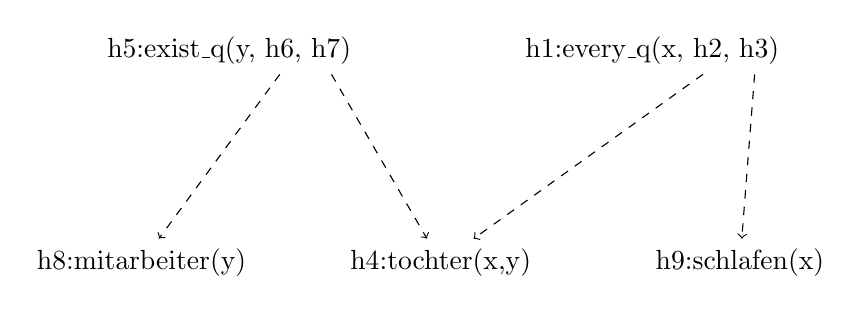
\begin{tikzpicture}[node distance=3.8cm]
\node(tochter) at (0,0){h4:tochter(x,y)};
\node(exist-q)[above left  of=tochter]{h5:exist\_q(y, h6, h7)};
\node(every-q)[above right of=tochter]{h1:every\_q(x, h2, h3)};
\node(mitarbeiter)[left of=tochter]{h8:mitarbeiter(y)};
\node(schlafen)[right of=tochter]{h9:schlafen(x)};
\draw[->,dashed]   (exist-q.-13) to (tochter);
\draw[->,dashed]   (every-q.-25) to (tochter);
\draw[->,dashed]   (exist-q.-25) to (mitarbeiter);
\draw[->,dashed]   (every-q.-13) to (schlafen);
\end{tikzpicture}
\caption{Dominanzverhältnisse für \emph{Jede Tochter eines Mitarbeiters schläft.}}\label{fig-Jede Tochter eines Mitarbeiters schläft-MRS}
\end{figure}
Die Restriktion des Allquantors ist h2 und h2 dominiert h4. Über den Body des Allquantors h3 wurde
nichts gesagt, aber da h2 schon belegt ist und die Variable von schlafen x ist, muss schlafen von h3
dominiert werden. Analog funktioniert das mit dem Existenzquantor: h6 dominiert die
mitarbeiter-Relation und da y ein Argument von tochter ist und der Existenzquantor sich auf y
bezieht, muss tochter von h7 dominiert werden. In Abbildung~\ref{fig-Jede Tochter eines Mitarbeiters
  schläft-MRS} ist nicht festgelegt, ob der Allquantor über dem Existenzquantor steht oder
andersherum. Entweder h2 wird mit h5
identifiziert und h3 mit h9 oder h6 wird direkt mit h8 identifiziert und h7 mit h1. Die Abbildungen~\ref{fig-Jede-Tochter-eines-Mitarbeiters-schläft-Allquantor} und~\ref{fig-Jede-Tochter-eines-Mitarbeiters-schläft-Existenzquantor} zeigen die entsprechend geskopten MRSen.
\begin{figure}
\begin{tikzpicture}[node distance=3.8cm,bezier bounding box]
\node(tochter) at (0,0){h4:tochter(x,y)};
\node(exist-q)[above left  of=tochter]{h5:exist\_q(y, h6, h7)};
\node(every-q)[above right of=tochter]{h1:every\_q(x, h2, h3)};
\node(mitarbeiter)[left of=tochter]{h8:mitarbeiter(y)};
\node(schlafen)[right of=tochter]{h9:schlafen(x)};
\draw   (exist-q.-12) to (tochter);
\draw   (every-q.-25) .. controls +(0,-2) and +(0,2).. (exist-q.north);
\draw   (exist-q.-25) to (mitarbeiter);
\draw   (every-q.-13) to (schlafen);
\end{tikzpicture}
\caption{Skopusaufgelöste MRS mit weitem Skopus für den Allquantor}\label{fig-Jede-Tochter-eines-Mitarbeiters-schläft-Allquantor}
\end{figure}
\begin{figure}
\begin{tikzpicture}[node distance=3.8cm,bezier bounding box]
\node(tochter) at (0,0){h4:tochter(x,y)};
\node(exist-q)[above left  of=tochter]{h5:exist\_q(y, h6, h7)};
\node(every-q)[above right of=tochter]{h1:every\_q(x, h2, h3)};
\node(mitarbeiter)[left of=tochter]{h8:mitarbeiter(y)};
\node(schlafen)[right of=tochter]{h9:schlafen(x)};
%\draw   (exist-q.-12) to (tochter);
\draw   (exist-q.-12) .. controls +(0,-1) and +(0,2).. (every-q.north);
\draw   (every-q.-25) to (tochter);
\draw   (exist-q.-25) to (mitarbeiter);
\draw   (every-q.-13) to (schlafen);
\end{tikzpicture}
\caption{Skopusaufgelöste MRS mit weitem Skopus für den Existenzquantor}\label{fig-Jede-Tochter-eines-Mitarbeiters-schläft-Existenzquantor}
\end{figure}
Die Skopus-aufgelösten MRSen entsprechen genau den beiden Lesarten aus (\ref{ex-Quantoren-Mitarbeiter-Tochter}).

Damit ist schon den wesentlichen Teil der Analyse erklärt. Es fehlt lediglich die Umsetzung
in Merkmalbeschreibungen für die entsprechenden Lexikoneinträge. 
(\mex{1}) zeigt den Lexikoneintrag für \emph{Tochter}:
\ea
\label{le-Tochter}%
\emph{Tochter}:\\
\ms{
cat & \ms{ head & \ms[noun]{
                  case & \type{nom}\\
                  }\\
           spr   & \nliste{ Det }\\
           comps & \nliste{ NP[\type{gen}]\ind{1} }\\
         }\\
cont & \ms{
       ltop & \ibox{2}\\
       ind  & \ibox{3}\\
       rels & \liste{ \ms[tochter\_rel]{
                      lbl  & \ibox{2}\\ 
                      arg0 & \ibox{3}\\ 
                      arg1 & \ibox{1}\\ 
                      } }\\
       hcons & \eliste
       }
}
\z
\emph{Tochter} verlangt einen Determinator und eine Genitiv-NP. Der Index der Genitiv-NP ist
identisch mit dem \argone der \type{tochter\_rel}"=Relation. Zum semantischen Beitrag sprachlicher
Zeichen gehört nicht nur ein Index, sondern auch ein \ltopm. \ltop steht dabei für \emph{local top}
und bezieht sich auf das lokal höchste Label. Oben wurde schon das Beispiel (\ref{ex-every-klein-kind-schlafen}) mit attributivem
Adjektiv besprochen. Der \ltopw eines Lexikoneintrags ist identisch mit dem Label der wichtigsten Relation, die von einem
Lexikoneintrag eingeführt wird (dem sogenannten \textsc{key}). Bei einfachen Beispielen wie dem
Adjektiv \emph{klein} und dem Nomen \emph{Tochter} gibt es ohnehin nur ein Element in \rels und
dessen Label ist dann identisch mit dem \ltop. Bei der Phrase \emph{kleinen Kinder}\label{page-kleinen-Kinder}, die oben schon
besprochen wurde, werden die \ltopwe von \emph{kleinen} und \emph{Kinder} identifiziert. Dadurch
ergeben sich die gemeinsamen Label"=Werte h2 in (\ref{ex-every-klein-kind-schlafen}).

(\mex{1}) zeigt den Lexikoneintrag für \emph{jede}:
\eas
Lexikoneintrag für \emph{jede}:\\
\ms{
cat & \ms{ head & \ms[det~~~~~~~~~~~~~~~~~~~~~~~~~~~~~~]{
                  case  \type{nom}\\
                  spec|cont \ms{ ltop & \ibox{1}\\
                                 ind  & \ibox{2}\\
                               }
                  }\\
           spr   & \eliste\\
           comps & \eliste\\
         }\\
cont & \ms{
       rels & \liste{ \ms[every\_q]{
                      arg0 & \ibox{2}\\ 
                      rstr & \ibox{3}\\ 
%                      body &\\
                      } }\\
       hcons & \liste{ \ms[qeq]{
                       harg & \ibox{3}\\
                       larg & \ibox{1}\\
                       }
               }\\
       }
}
\zs
\emph{jede} ist ein Determinator, der selbst keine Argumente braucht, also eine leere \spr- und
\compsl hat. Der Allquantor wird in der \relsl eingeführt. \argzero ist das Merkmal für die
Variable. Außerdem gibt es je ein Merkmal für die Restriktion und den Body. Für die Restriktion
wurde oben angenommen, dass sie in einer \qeq\vspace{-2pt}\hspace{-.5ex}\hyp Relation zum Handel der \nbar steht. Das Nomen kann
zwar über die \sprl auf den Determinator zugreifen, aber andersrum ist das nicht
möglich. Determinatoren sind vollständig und somit ist ein Zugriff auf das Nomen über Valenzmerkmale
nicht möglich. Man behilft sich deshalb mit einem Trick: Analog zum \modm nimmt man ein
\textsc{spec}"=Merkmal an \citep[\page 50--51]{ps2}. \textsc{spec} steht für \emph{specified}. Der Wert des \specms ist
entweder vom Typ \type{none} oder vom Typ \type{sign}. Über den \specw kann man auf den \ltopw und
den Index des Nomens zugreifen, das mit einem Determinator kombiniert wird. So wird es möglich
aufzuschreiben, dass die Restriktion des Allquantors \qeq\vspace{-2pt} mit dem \ltopw der \nbar
ist. Das \textsc{h} in \textsc{harg} steht dabei für \emph{hole}, also die Stelle, in die etwas
eingestöpselt werden kann, und das \textsc{l} in \textsc{larg} steht für \emph{label}. Für unser
Beispiel \emph{jede Tochter} bedeutet das, dass \type{tochter\_rel} in die Restriktion von
\emph{every\_q} eingestöpselt werden kann oder irgendein Quantor, der \type{tochter\_rel}
dominiert. Der \textsc{body}"=Wert des Quantors wird einfach nicht angegeben. Das ist Teil der
Unterspezifikation: Irgendein Handle einer anderen Relation oder eines anderen Quantors kann dort
eingefügt werden, Hauptsache zum Schluss sind alle Variablen im Bereich eines Quantors und keins der
Handle"=Constraints ist verletzt.

Abbildung~\ref{fig-Jede-Tochter-eines-Mitarbeiters-schläft} zeigt die Analyse unseres Beispiels.
\begin{figure}
\begin{sideways}
%\centerfit{%
\scalebox{.9}{%
\begin{forest}
sm edges
[V\feattab{\rels \nliste{ h1:every(x,h2,h3), h4:tochter(x,y), h5:exist(y,h6,h7), h8:mitarbeiter(y),
    h9:schlafen(x) },\\
               \hcons \nliste{ h2 \qeq h4, h6 \qeq h8 }}
  [NP\feattab{\rels \nliste{ h1:every(x,h2,h3), h4:tochter(x,y), h5:exist(y,h6,h7), h8:mitarbeiter(y) },\\
               \hcons \nliste{ h2 \qeq h4, h6 \qeq h8 }}
    [Det\feattab{\rels \nliste{ h1:every(x,h2,h3) },\\
               \hcons \nliste{ h2 \qeq h4 }} [jede] ]
    [N\feattab{\rels \nliste{ h4:tochter(x,y), h5:exist(y,h6,h7), h8:mitarbeiter(y) },\\
               \hcons \nliste{ h6 \qeq h8 }}
      [N\feattab{\rels \nliste{ h4:tochter(x,y) },\\
                 \hcons \eliste} [Tochter] ]
      [NP\feattab{\rels \nliste{ h5:exist(y,h6,h7), h8:mitarbeiter(y) },\\
                  \hcons \nliste{ h6 \qeq h8 }} 
         [Det\feattab{\rels \nliste{ h5:exist(y,h6,h7) },\\
                      \hcons \nliste{ h6 \qeq h8 }} [eines]]
         [N\feattab{\rels \nliste{ h8:mitarbeiter(y) },\\
                    \hcons \eliste} [Mitarbeiters]] ] ] ]
   [V\feattab{\rels \nliste{ h9:schlafen(x) },\\
              \hcons \eliste} [schläft]]]
\end{forest}
}
\end{sideways}
\caption{\label{fig-Jede-Tochter-eines-Mitarbeiters-schläft}Analyse des Beispiels \emph{Jede Tochter
    eines Mitarbeiters schläft.}}
\end{figure}
Wie im Abschnitt~\ref{sec-Komposition} erklärt werden die Relationen einfach durch Listenverkettung von den
Töchtern zum Mutterknoten hochgereicht. Genauso funktioniert das für die Handle"=Constraints:
\ea
\type{phrase} \impl\\
\onems{
cont|hcons  \normalfont collect-hcons(\ibox{1})\\
dtrs  \ibox{1} \\
}
\z

\noindent
Zum \specw gibt es noch etwas zu erklären. Ich hatte gesagt, dass das \specm analog zum \modm ist,
aber das stimmt nicht ganz. Das \modm ähnelt den Valenzmerkmalen. Es gibt das Kopf"=Adjunkt"=Schema,
in dem der \modw der Nichtkopftochter mit der Kopftochter identifiziert wird. Das \specm wird dazu
benötigt, von innerhalb der Nicht"=Kopftochter bei Bedarf auf Eigenschaften der Kopftochter
zugreifen zu können. In der hier vorgestellten Grammatik scheint es so zu sein, dass diese Situation nur
für Determinatoren vorliegt und also nur für Determinatoren ein \specm annehmen und dieses in
Kopf"=Spezifikator"=Strukturen mit der Kopftochter identifizieren. Es gibt aber auch in
Präpositionalphrasen die Möglichkeit einen Spezifikator zu haben. Die Duden"=Grammatik \citeyearpar[\S 1300]{Duden2005} gibt Beispiele wie die in (\mex{1}):
\eal
\ex {}[[Einen Schritt] vor dem Abgrund] blieb er stehen.\label{Beispiel-Schritt-vor-dem-Abgrund}
\ex {}[[Kurz] nach dem Start] fiel die Klimaanlage aus.
\ex {}[[Schräg] hinter der Scheune] ist ein Weiher.
\ex {}[[Mitten] im Urwald] stießen die Forscher auf einen alten Tempel.
\zl
Präpositionen können durch eine Nominalphrase oder eine Adjektivphrase spezifiziert werden. Wie bei
Determinatoren auch, darf es nur ein spezifizierendes Element geben:
\eal
\ex[*]{
[\sub{PP} einen Schritt [\sub{PP} kurz [\sub{PP} vor dem Abgrund]]]
}
\ex[*]{
[\sub{PP} kurz [\sub{PP} einen Schritt [\sub{PP} vor dem Abgrund]]]
}
\zl
Es ist also sinnvoll, diese zusätzlichen Elemente als Spezifikatoren zu analysieren.
Somit muss man also Kopf"=Spezifikator"=Strukturen mit Zugriff des Spezifikators auf den Kopf von
solchen ohne Zugriff unterscheiden. Das kann man mithilfe das folgenden Prinzips:

\begin{prinzip-break}[Spezifikatorprinzip (\textsc{spec}-Principle)] 
\label{prinzip-spec}\is{Prinzip!Spezifikator-}
Wenn eine Tochter, die keine Kopf"|tochter ist, in einer Kopf"|struktur
einen von \type{none} verschiedenen \textsc{spec}-Wert besitzt, so ist dieser token-identisch mit
%dem \textsc{synsem}-Wert 
der Kopf"|tochter.
\end{prinzip-break}
Formalisieren lässt sich das Prinzip wie folgt:
\ea
\ms{ non-head-dtrs & \liste{ [\textsc{head|spec} \type{sign}] } } \impl
\ms{ head-dtr & \ibox{1}\\
     non-head-dtrs & \liste{ [\textsc{head|spec} \ibox{1}] } }
\z

\subsection{Eigennamen, Pronomen, Possessivpronomen}

In der Prädikatenlogik gibt es Individuenkonstanten. Das bedeutet, dass man für ein bestimmtes
Diksursuniversum sagt, dass ein bestimmter Bezeichner einer bestimmten Entität zugeordnet wird. Es
gibt ein Objekt, das den Bezeichner \emph{Aicke} bekommt \citep[68]{AAD73a}. In dem hier
vorliegenden Fragment wird das anders gemacht. Es wird als Eigenschaft einer bestimmten Entität
angesehen, dass sie oder er \emph{Aicke} heißt. Die Repräsentation mittels Relationen erfolgt
parallel zu der von Nominalphrasen mit Determinator. (\mex{1}) zeigt den Lexikoneintrag für den
Eigennamen \emph{Aicke}:
\eas
Lexikoneintrag für \emph{Aicke}:\\
\ms{
cat & \ms{ head & noun\\
           spr   & \eliste\\
           comps & \eliste\\
         }\\
cont & \ms{
       ltop & \ibox{1}\\
       ind  & \ibox{2} \ms{
                       per & 3\\
                       num & sg\\
                       }\\ 
       rels & \liste{ \ms[proper\_q]{
                      arg0 & \ibox{2}\\ 
                      rstr & \ibox{3}\\ 
%                      body &\\
                      }, \ms[named\_rel]{
                         lbl & \ibox{1}\\
                         arg0 & \ibox{2}\\
                         name & "`Aicke"'~~\\
                         } }\\
       hcons & \liste{ \ms[qeq]{
                       harg & \ibox{3}\\
                       larg & \ibox{1}\\
                       }
               }\\
       }
}
\zs
Damit ist der Eigenname \emph{Aicke} komplett parallel zu einer NP wie \emph{die Person}. Das
Problem, das es noch zu lösen gilt, ist, dass Eigennamen normalerweise eindeutig referieren. Deshalb
werden in der Prädikatenlogik ja auch Individuenkonstanten verwendet. Diese interagieren nicht mit
Quantoren. Die Repräsentation in (\mex{0}) legt aber genau eine solche Interpretation nahe. Durch
die Verwendung von Handle"=Constraints können andere Quantoren zwischen proper\_q und named\_rel
skopen. Das kann man ausschließen, indem man die named\_rel direkt bei proper\_q einstöpselt:
\eas
Lexikoneintrag für \emph{Aicke}:\\
\ms{
cat & \ms{ head & noun\\
           spr   & \eliste\\
           comps & \eliste\\
         }\\
cont & \ms{
       ltop & \ibox{1}\\
       ind  & \ibox{2} \ms{
                       per & 3\\
                       num & sg\\
                       }\\ 
       rels & \liste{ \ms[proper\_q]{
                      arg0 & \ibox{2}\\ 
                      rstr & \ibox{1}\\ 
%                      body &\\
                      }, \ms[named\_rel]{
                         lbl & \ibox{1}\\
                         arg0 & \ibox{2}\\
                         name & "`Aicke"'\\
                         } }\\
       hcons & \eliste\\
       }
}
\zs
Das hätte dann zur Folge, dass andere Quantoren immer Skopus über Ausdrücke mit Eigennamen
haben. Welche der beiden Analysen sinnvoll ist, hängt von weiteren Beschränkungen in Bezug auf den
Aufbau von MRS bzw.\ Regeln für die Interpretation von MRSen zusammen. Man muss irgendwie erreichen, dass \ibox{2} sich
in einem gegebenen Diskursuniversum auf genau ein Objekt bezieht, so wie das bei
Individuenkonstanten in der Prädikatenlogik eben auch der Fall ist.

Die Situation für Pronomina ist ähnlich. Es gibt eine Art Quantor für Pronomina und eine
entsprechende Relation. Der Eintrag für das Pronomen \emph{er} von Seite~\pageref{le-er} kann nun wie folgt um die \rels- und \hconswe
erweitert werden:
\eas
Lexikoneintrag für \emph{er}:\\
\ms{ 
  cat & \ms{ head  & \ms[noun]{
                     case & nom\\
                     }\\
             spr   & \eliste\\
             comps & \eliste \\
           } \\
  cont &  \ms{
       ltop & \ibox{1}\\
       ind  & \ibox{2} \ms{
                       per & 3\\
                       num & sg\\
                       gen & mas \\
                      }\\ 
       rels & \liste{ \ms[pronoun\_q]{
                      arg0 & \ibox{2}\\ 
                      rstr & \ibox{3}\\ 
%                      body &\\
                      }, \ms[pronoun\_rel]{
                         lbl & \ibox{1}\\
                         arg0 & \ibox{2}\\
                         } }\\
       hcons & \liste{ \ms[qeq]{
                       harg & \ibox{3}\\
                       larg & \ibox{1}\\
                       }
               }\\
           } \\
}
\zs
Die Annahme einer pronoun\_rel"=Relation ist unschön, weil man nicht sagen kann, in welchen
Diskursuniversen diese wahr sein soll, aber diese Relation ist auch dem allgemeinen Format mit
Quantoren und gebundenen Variablen geschuldet.

Als letztes in diesem Abschnitt sollen Possessivpronomen diskutiert werden. Diese sind interessant,
weil sie eine Mischung aus Determinatoren und Pronomen sind. (\mex{1}) zeigt ein Beispiel:
\ea
ihr Buch
\z
Den Lexikoneintrag für \emph{ihr} zeigt (\mex{1}):
\eas
Lexikoneintrag für \emph{ihr}:\\
\ms{ 
  cat & \ms{ head  & \ms[det]{
                     case & nom\\
                     spec & \ms{ cont & \ms{ ltop & \ibox{1}\\
                                             ind  & \ibox{2}\\
                                           }}\\
                     }\\
             spr   & \eliste\\
             comps & \eliste \\
           } \\
  cont &  \ms{
       ltop & \ibox{3}\\
       ind  & \ibox{4} \ms{
                       per & 3\\
                       num & sg\\
                       gen & fem\\
                      }\\ 
       rels & \liste{ \ms[def\_q]{
                      arg0 & \ibox{2}\\ 
                      rstr & \ibox{5}\\ 
%                      body &\\
                      }, \ms[besitzen\_rel]{
                            lbl  & \ibox{1}\\     % pronoun_q(x,h, h) h1:pronoun_rel(x),
                                % h1:besitzen(x,y) ^ h1:buch(y)
%                           arg0 & event\\
                            arg1 & \ibox{4}\\
                            arg2 & \ibox{2}
                      }, \ms[pronoun\_q]{
                         arg0 & \ibox{4}\\
                         rstr & \ibox{6}\\
                      }, \ms[pronoun\_rel]{
                         lbl & \ibox{3}\\
                         arg0 & \ibox{4}\\
                         } }\\
       hcons & \liste{ \ms[qeq]{
                       harg & \ibox{5}\\
                       larg & \ibox{1}\\
                       },
                       \ms[qeq]{
                       harg & \ibox{6}\\
                       larg & \ibox{3} }
               }\\
           } \\
}
\zs
% ERG verwendet def_implicit_q_rel für Possessivpronomina.
% def_implicit_q_rel := def_q_rel & implicit_q_rel.
Kombiniert man \emph{ihr} mit \emph{Buch} erhält man die folgende MRS:
\ea
\textmrs{ h0, \{ h1:def\_q(x, h2, h3), h4:besitzen(e1,y,x), h4:buch(x),
             h5:pronoun\_q(y, h6, h7), \hphantom{\textlangle~}h8:pronoun\_rel(y) \},\\
\hphantom{\textlangle~}\{ h2 \qeq h4, h6 \qeq h8 \}  }
\z
Das Possessivpronomen verhält sich wie ein definiter Artikel und die Restriktion des entsprechenden
Quantors def\_q h2 ist \qeq mit dem Handle der besitzen"=Relation h4, das mit dem Handel von
\emph{Buch} identifiziert ist. Außerdem gibt es den Quantor für das feminine Pronomen, das sich auf
die Besitzende bezieht und das \argone der besitzen"=Relation und das Argument der zum Quantor gehörenden pronoun\_rel ist.

Man beachte, dass der Index des Possessivpronomens sich vom Index der \nbar unterscheidet, mit der
das Pronomen kombiniert wird.

\subsection{\emph{mutmaßliche Mörder}}

Bisher waren die Regeln zur semantischen Komposition sehr einfach. Es wurden einfach die \relslen
verknüpft und die \ltopwe identifiziert. Damit kann man die Verhältnisse in (\mex{1}) aber nicht erfassen.

\ea
\label{soldat}
%% Darin heißt es, dass "Soldaten nicht nur potentielle Mörder sind, sondern im wahrsten Sinne des Wortes bezahlte Killer".21.10.1994 taz Inland 97 Zeilen, hans-hermann kotte S. 5
%% Augst hatte 1989 bei einer Diskussion Soldaten als "potentielle Mörder" bezeichnet. 10.10.1994 taz Aktuelles 14 Zeilen, S. 2

%% Er hatte sich in einem Leserbrief mit dem Ausspruch "Alle Soldaten sind potentielle Mörder" solidarisiert.22.9.1994 taz Tagesthema 91 Zeilen, kotte S. 3
Gewalt provoziere immer Gegengewalt und: "`Soldaten sind potentielle Mörder."'\footnote{
23.12.1993, taz berlin, S.\,18.
}
\z
Die Formel in (\mex{1}) wäre für die Repräsentation des Prädikates im Satz (\mex{2}) angemessen, für
die Prädikation in (\mex{0}) ist sie es nicht.
\ea
\relation{mörder}(x)
\z
\ea
Soldaten sind Mörder.\footnote{
  Tucholsky, Kurt, (1931), "`Der bewachte Kriegsschauplatz"', \emph{Die Weltbühne}, S.\,31.
}
\z
Genauso gilt bis zur rechtskräftigen Verurteilung von Mördern, dass man sie nicht Mörder nennen
darf, sondern von mutmaßlichen Mördern reden muss. 

Auf S.\,\pageref{page-kleinen-Kinder} wurde bereits die Kombination von \emph{kleinen} und
\emph{Kinder} besprochen. Dabei wird der \ltopw des modifizierten Nomens mit dem \ltopw des
Adjektivs identifiziert. (\mex{1}) zeigt den Lexikoneintrag für das Adjektiv \emph{kleinen}:
\eas
\label{le-kleinen-vorläufig}%
Lexikoneintrag für \emph{kleinen} (vorläufig):\\
\ms{
cat & \ms{ head & \ms[adj]{
                  mod & \ms{ cat & \ms{ head & noun\\
                                        spr  & \nliste{ Det }\\
                                        comps & \eliste }\\
                             cont & \ms{ ltop & \ibox{1}\\
                                         ind  & \ibox{2}\\
                                       }}}\\
           spr & \eliste\\
           comps & \eliste\\
         }\\
cont & \ms{ ltop & \ibox{1}\\
            ind  & \ibox{2}\\
            rels & \liste{ \ms[klein]{
                           lbl  & \ibox{1}\\ 
                           arg0 & \ibox{2}\\
                           } }\\
            hcons & \eliste\\
          }\\
}
\zs
In (\mex{0}) wird der \ltopw des modifizierten Nomens mit dem \ltopw des Adjektivs
identifiziert. Für die potentiellen Mörder wäre das falsch, denn sie sind nicht potentiell und
Mörder (\mex{1}b), stattdessen muss das \emph{potentiell} den \emph{Mörder} wie in (\mex{1}c) einschließen.
\eal
\ex \textmrs{ h0, \{ h1:klein(x), h1:mörder(x) \}, \{  \}  }
\ex \textmrs{ h0, \{ h1:potentiell(x), h1:mörder(x) \}, \{  \}  }
\ex\label{mrs-potentielle-Mörder}
\textmrs{ h0, \{ h1:potentiell(h2), h2:mörder(x) \}, \{  \}  }
\zl

Für das Adjektiv \emph{potentielle} ergibt sich:
\eas
Lexikoneintrag für \emph{potentielle}:\\
\ms{
cat & \ms{ head & \ms[adj]{
                  mod & \ms{ cat & \ms{ head & noun\\
                                        spr  & \nliste{ Det }\\
                                        comps & \eliste }\\
                             cont & \ms{ ltop & \ibox{1}\\
                                         ind  & \ibox{2}\\
                                       }}}\\
           spr & \eliste\\
           comps & \eliste\\
         }\\
cont & \ms{ ltop & \ibox{3}\\
            ind  & \ibox{2}\\
            rels & \liste{ \ms[potentiell]{
                           lbl  & \ibox{3}\\
                           arg0 & \ibox{1}\\
                           } }\\
            hcons & \eliste\\
          }\\
}
\zs

Wie man an (\ref{mrs-potentielle-Mörder}) sehen kann muss der \ltopw einer Kopf"=Adjunkt"=Struktur
durch die Adjunkttochter bestimmt werden, denn \ltop ist das Label des jeweils einbettenden
Prädikats. Bei intersektiven Adjektiven wie \emph{klein} sind beide Handels identifiziert, weshalb
auch da der \ltopw von der Adjunkttochter genommen werden kann. Die folgende Beschränkung gilt also
zusätzlich zu den bereits beschrieben Beschränkungen für Kopf"=Adjunkt"=Strukturen:
\ea
\type{head-adjunct-phrase} \impl
  \ms{ cont|ltop & \ibox{1}\\
       non-head-dtrs & \liste{ \ms{ cont|ltop & \ibox{1} } }\\
     }
\z

Anhand von Adjektiven wie \emph{potentiell} kann man sich klarmachen, warum Determinatoren auf das Label der
modifizierten \nbar zugreifen können müssen und weshalb man also das \specm braucht. Man könnte ja
vermuten, dass man statt dessen vom Nomen auf den Determinator zugreifen kann und
Skopusrestriktionen beim Nomen kodieren kann. Im Lexikoneintrag für \emph{Mörder} kann man zwar
auf das Label von einem Determinator zugreifen, weil dieser in der \sprl repräsentiert ist und man
kennt auch das Label des Nomens selbst. Es wäre also möglich, innerhalb des Lexikoneintrags des
Nomens das Label des Determinators mittels \qeq zum Label des Nomens in Beziehung zu setzen. Das
reicht aber nicht aus, weil es Adjektive wie \emph{potentiell} gibt. Im Lexikoneintrag des Nomens
kann man nicht wissen, was das höchste Label in der \nbar sein wird. Wird es einbettende Adjektive
wie \emph{potentiell} geben? Oder nur Adjektive wie \emph{kleine}? Oder gar keine Adjektive? Man
muss also die komplette \nbar kennen und deren \ltopw für ein Handle"=Constraint im Lexikoneintrag
des Determinators verwenden. 

\subsection{\emph{glauben} und Einhörner}

Im letzten Abschnitt ging es um Adjunkte, die Skopus über Elemente haben können, die sie
modifizieren, aber auch bei Komplementen kann das der Fall sein. Der folgende Satz hat drei Lesarten:
\ea
Alle Affen glauben, dass ein Einhorn schläft.
\z
Es kann sein, dass es kein Einhorn gibt und nur die Affen glauben, dass es etwas gibt, das ein
Einhorn ist und schläft. Außerdem kann es sein, dass es ein bestimmtes Einhorn gibt, von dem alle
Affen glauben, dass es schläft. Und dann kann es sein, dass es für jeden Affen ein Einhorn gibt, von
dem er glaubt, dass es schläft. (\mex{1}) zeigt die drei Lesarten im Überblick:
\eal
\label{ex-Prädikatenlogik-alle-Affen-glauben-dass-ein-Einhorn-schläft}
\ex $\forall$x \relation{affe}(x) $\to$ \relation{glauben}($\exists$y \relation{einhorn}(y) $\wedge$ schlafen(y))
\ex $\exists$y \relation{einhorn}(y) $\wedge$ ($\forall$x \relation{affe}(x) $\to$ \relation{glauben}(schlafen(y)))
\ex $\forall$x \relation{affe}(x) $\to$ ($\exists$y \relation{einhorn}(y) $\wedge$ \relation{glauben}(schlafen(y)))
\zl
In der hier verwendeten Notation mit den Quantoren als dreistelliger Relation sieht das wie folgt aus:
\eal
\label{ex-Quantoren-Relationen-alle-Affen-glauben-dass-ein-Einhorn-schläft}
\ex every\_q(x, affe(x), glauben(exist\_q(y, einhorn(y), schlafen(y))))
\ex exist\_q(y, einhorn(y), every\_q(x,affe(x), glauben(schlafen(y)))
\ex every\_q(x, affe(x), exist\_q(y, einhorn(y), glauben(schlafen(y)))
\zl
Letztendlich ergeben sich diese Lesarten in der hier beschriebenen Grammatik fast von selbst. Die
beiden Lesarten mit Skopus oberhalb von \emph{glauben} sind nach allem, was bisher gesagt wurde,
erwartet. Erklärt werden muss, warum der Existenzquantor zwischen \emph{glauben} und \emph{schlafen}
skopen kann. Das kann erreicht werden, indem man nicht \relation{schlafen} direkt zum Argument von
\relation{glauben} macht, sondern ein Handle"=Argument zum Label von \relation{schlafen} in
\qeq-Relation setzt. Die MRS, die benötigt wird, zeigt (\mex{1}):
\ea
\textmrs{ h0, \{ h1:every\_q(x, h2, h3), h4:affe(x), h5:glauben(e1, x, h6), h7:exist\_q(y, h8, h9), \\
             \hphantom{\textlangle~}h10:einhorn(y), h11:schlafen(e2, y) \},\\
\hphantom{\textlangle~}\{ h2 \qeq h4, h6 \qeq h11, h9 \qeq h10 \}  }
\z
Den entsprechenden Lexikoneintrag für \emph{glauben} zeigt (\mex{1}):
\eas
\label{le-glauben}%
Lexikoneintrag für \emph{glauben}:\\
\ms
{ cat & \ms{ head & \ms[verb]
                     { vform & fin \\} \\
             arg-st & \liste{ NP[\type{nom}]\ind{1}, CP[\type{dass}, \ltop \ibox{2}]   } \\
           } \\
  cont &  \ms{
          ind & \ibox{4} event\\
          rels & \liste{ \ms[glauben]{ 
                          arg0 & \ibox{4}\\
                          arg1 & \ibox{1} \\
                          arg2 & \ibox{3} \\
                          } }\\
          hcons & \liste{ \ms[qeq]{
                          harg & \ibox{3}\\
                          larg & \ibox{2}} } }\\
}
% \avm{
% [ cat & [ head & [\type*{verb}
%                   vform & fin ] \\
%           arg-st & < NP[\type{nom}]\ind{1}, CP[\type{dass}, \ltop \ibox{2}] > \\
%            ] \\
%   cont & [ind  & \ibox{4} event\\
%           rels & < [\type*{glauben}\\ 
%                     arg0 & \ibox{4}\\
%                     arg1 & \ibox{1}\\
%                     arg2 & \ibox{3} ] >\\
%           hcons & < [\type*{qeq}
%                      harg & \ibox{3}\\
%                      larg & \ibox{2} ] > ] ]
% } 
\zs
Während bei Verben wie \emph{geben} (siehe (\ref{le-gibt} auf S.\,\pageref{le-gibt}) die \hconsl leer ist, gibt es bei \emph{glauben} ein
\qeq-Element. \argtwo von \relation{glauben} wird in Beziehung zum \ltopw des CP"=Arguments
gesetzt. Da die beiden Werte nicht identifiziert werden, sondern lediglich eine Dominanzrelation
festgelegt wird, kann der Existenzquantor zwischen \relation{glauben} und \relation{schlafen}
skopen. Mit diesem Lexikoneintrag erhalten wir die Dominanzverhältnisse in
Abbildung~\ref{fig-alle-Affen-glauben-dass-ein-Einhorn-schläft} und diese erlauben genau die drei
Lesarten, die in (\ref{ex-Prädikatenlogik-alle-Affen-glauben-dass-ein-Einhorn-schläft}) bzw.\
(\ref{ex-Quantoren-Relationen-alle-Affen-glauben-dass-ein-Einhorn-schläft}) angegeben wurden.

\begin{figure}
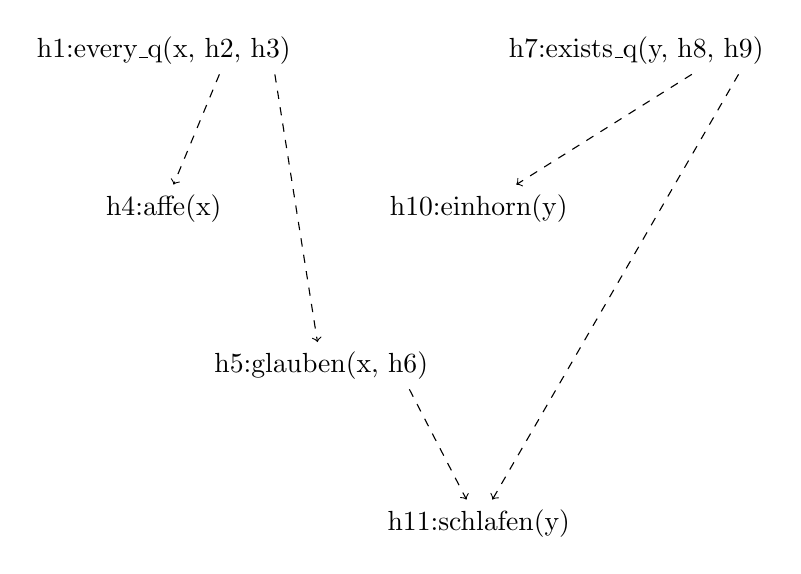
\begin{tikzpicture}
%\draw (-5,10) to[grid with coordinates] (5,-.5);
\node(schlafen) at (0,0) {h11:schlafen(y)};
\node(glauben)  at (-2,2){h5:glauben(x, h6)};
\node(affe)     at (-4,4){h4:affe(x)};
\node(einhorn)  at (0,4) {h10:einhorn(y)};
\node(every-q)  at (-4,6){h1:every\_q(x, h2, h3)};
\node(exists-q) at (2,6) {h7:exists\_q(y, h8, h9)};

\draw[->,dashed]   (every-q.-23)  to (affe);
\draw[->,dashed]   (every-q.-12)  to (glauben);
\draw[->,dashed]   (exists-q.-23) to (einhorn);
\draw[->,dashed]   (exists-q.-13) to (schlafen);
\draw[->,dashed]   (glauben.-15)  to (schlafen);
\end{tikzpicture}
\caption{Dominanzgraph für \emph{Alle Affen glauben, dass ein Einhorn schläft.}}\label{fig-alle-Affen-glauben-dass-ein-Einhorn-schläft}

\end{figure}

\subsection{\emph{scheinbar einfache Beispiele}}
\label{sec-scheinbar-einfaches-Beispiel}

Beispiele wie die in (\mex{1}) sind scheinbar einfach:
\ea
\label{ex-ein-scheinbar-einfaches-Beispiel}
ein scheinbar einfaches Beispiel
\z
In der früheren situationssemantischen Analyse von Adjektiven war das Beispiel in (\mex{0}) aber
wirklich nur scheinbar einfach. In Wirklichkeit war es vertrackt. Bob \citet{Kasper97a} hat darauf hingewiesen,
dass es bei der Analyse von Beispielen wie (\mex{0}) ein Problem gibt, wenn \emph{scheinbar} den
semantischen Beitrag von \emph{einfaches Beispiel} einbettet.\footnote{%
 Leider wurde dieser großartige Artikel nie veröffentlicht. Eine Variante der Analyse Kaspers
 findet man in \citew[Abschnitt~4.3]{Mueller99a}. \citet[Section~3.2]{KR2024a} diskutieren sie im Semantik"=Kapitel des HPSG"=Handbuches.
} Man bekäme eine Repräsentation, in der sowohl \emph{einfaches} als auch \emph{Beispiel} unter
\emph{scheinbar} eingebettet wäre. Das heißt, die semantische Repräsentation wäre die, die man für
(\mex{1}) erwarten würde:
\ea
ein scheinbares einfaches Beispiel
\z
In der Welt der MRS entspräche das der Repräsentation in (\mex{1}a). Was man jedoch für (\ref{ex-ein-scheinbar-einfaches-Beispiel}) braucht ist die in (\mex{1}b):

\eal
\ex \textmrs{ h0, \{ h1:exist\_q(x, h2, h3), h4:scheinbar(h5), h6:einfach(x), h6:beispiel(x) \},\\
    \hphantom{\textlangle~}\{ h2 \qeq h4, h5 \qeq h6 \}  }
\ex
\label{mrs-ein-scheinbar-einfaches-Beispiel} 
\textmrs{ h0, \{ h1:exist\_q(x, h2, h3), h4:scheinbar(h5), h6:einfach(x), h4:beispiel(x) \},\\
    \hphantom{\textlangle~}\{ h2 \qeq h4, h5 \qeq h6 \}  }
\zl

\noindent
In (\mex{0}b) wird über das Beispiel gesagt, dass es scheinbar einfach ist. In (\mex{0}a) wird
dagegen über etwas, das einfach und ein Beispiel ist, gesagt, dass es scheinbar ist. Bei der bisher
entwickelten Analyse würde aber nicht die nur falsche MRS in (\mex{0}a) herauskommen, sondern die
sich ergebende MRS wäre auch noch inkonsistent:
\ea
\textmrs{ h0, \{ h1:exist\_q(x, h2, h3), h4:scheinbar(h5), h4:einfach(x), h4:beispiel(x) \},\\
    \hphantom{\textlangle~}\{ h2 \qeq h4, h5 \qeq h4 \}  }
\z
Da h5 \qeq h4 gilt und h4 aber auch das Label von h4:scheinbar(h5) ist, dominiert scheinbar sich
selbst, eine unzulässige Konfiguration.

Die Lösung für das Problem besteht darin, dass der \ltopw eines intersektiven Adjektivs nicht mehr
im Lexikoneintrag mit dem des modifizierten Nomens identifiziert wird \citep[Section~6.3]{CFPS2005a}. 
\eas
Lexikoneintrag für \emph{kleinen}:\\% (vorläufig):\\
\ms{
cat & \ms{ head & \ms[adj]{
                  mod & \ms{ cat & \ms{ head & noun\\
                                        spr  & \nliste{ Det }\\
                                        comps & \eliste }\\
                             cont & \ms{ %ltop & \ibox{1}\\
                                         ind  & \ibox{2}\\
                                       }}}\\
           spr & \eliste\\
           comps & \eliste\\
         }\\
cont & \ms{ ltop & \ibox{1}\\
            ind  & \ibox{2}\\
            rels & \liste{ \ms[klein]{
                           lbl  & \ibox{1}\\ 
                           arg0 & \ibox{2}\\
                           } }\\
            hcons & \eliste\\
          }\\
}
\zs
Im Gegensatz zu (\ref{le-kleinen-vorläufig}) wird der \ltopw in (\mex{0}) nicht mit dem \ltopw innerhalb des \modwes gleichgesetzt.
Stattdessen wird festgelegt, dass in Kopf"=Adjunkt"=Strukturen mit nicht-skopalen Adjunkten die \ltopwe der Töchter identifiziert
werden. 
\ea
\label{ex-scopal-ltop}
\avm{
[ non-head-dtrs < [ cat|head|scopal & minus ] > ]} \impl
\flushright 
\avm{[ head-dtr|cont|ltop & \1\\
  non-head-dtrs < [ cont|ltop & \1 ] > ]
}
\z
% bug
\medskip

\noindent
Das bedeutet, dass die Handels von \emph{einfach} und \emph{Beispiel} nicht im
Lexikoneintrag von \emph{einfaches} gleichgesetzt werden, dass aber die \ltopwe von \emph{scheinbar
  einfaches} und \emph{Beispiel} durch das Kopf"=Adjunkt"=Schema identifiziert werden. Damit ergibt
sich die richtige MRS in (\ref{mrs-ein-scheinbar-einfaches-Beispiel}), weil der \ltopw von
\emph{scheinbar} mit dem von \emph{Beispiel} gleichgesetzt wird, denn \emph{scheinbar} steuert
den \ltopw von \emph{scheinbar einfaches} bei.

Es stellt sich die Frage, ob es gut ist, die Tatsache, dass es um skopale oder intersective
Modifikatoren geht als Kopfmerkmal zu repräsentieren. Die Alternative bestünde darin, die
Hauptrelation des Kopfes zu kennzeichnen und dann bei Modifikation als Antezedens einer Implikation
auf das Vorliegen einer skopalen oder intersektionalen Relation zu testen. Die Repräsentation als
Kopfmerkmal scheint die richtigen Vorhersagen bezüglich Koordinierbarkeit zu machen:
\eal
\ex[*]{
ein mutmaßlicher und brutaler Mörder
}
\ex[]{
ein mutmaßlicher brutaler Mörder
}
\ex[]{
ein brutaler mutmaßlicher Mörder
}
\zl


Damit ist die Einführung in die Minimal Recursion Semantics abgeschlossen. Es freut mich, dass Sie
die Warnung zu Beginn dieses Abschnitts ignoriert und auch diesen technischen Teil gelesen haben.

% Fragen:
%
% LTOP bei SPR und COMPS identifizieren? Wozu?
% Wenn man das täte, müsste man Verben wie glauben anders behandeln, denn deren LTOP ist nicht mit
% dem des Komplements identifizierbar, denn es bettet das LTOP ein.


\section{Alternativen}

\subsection{Intersektive und skopale Modifikatoren}

\citet*{CFPS2005a} skizzieren eine Typhierarchie, die die korrekte Weitergabe von \ltopwen
sicherstellen soll. Sie haben ausdrücklich angemerkt, dass das nur eine Skizze ist, aber ich möchte
hier dennoch einige Gründe dafür anführen, warum dieser Vorschlag formal nicht funktioniert, also
auch keine Skizze mit noch auszufüllenden Details sein kann. Das kann letztendlich für ein tieferes
Verständnis von HPSG und den allgemein zur Verfügung stehenden Mechanismen hilfreich
sein. Abbildung~\ref{fig-skopal-intesaktiv-MRS-Paper} zeigt eine Hierarchie von Typen mit
entsprechenden Beschränkungen, wie sie von \citet[\page 308]{CFPS2005a} angegeben wird.
\begin{figure}
\begin{forest}
type hierarchy
[\avm{[\type*{phrase}
       cont  [ hook & \1 [ gtop & \0 ]\\
                rels & \2 \+ \3\\
                hcons & \4 \+ \5 ]\\
       dtr1|cont [ hook & \1\\
                   rels & \2\\
                   hcons & \4]\\ 
       dtr2|cont [ hook & [ gtop & \0 ]\\
                   rels & \2\\
                   hcons & \4]]}   
  [\avm{[\type*{intersective-phrase}
         dtr1|cont|hook|ltop & \6\\
         dtr2|cont|hook|ltop & \6]}]
  [\avm{[\type*{scopal-phrase}
         dtr1|cont & [ hook & [ltop & \7]\\
                       rels & < \ldots{} [\type*{scopal-reln} 
                                         lbl & \7\\
                                         arg1 & \8] ~\ldots{} >\\
                       hcons & < [\type*{qeq}
                                  harg & \8\\
                                  larg & \9], \ldots > ]\\
         \punk{dtr2|cont|hook|ltop}{\9}]}]]
\end{forest}
\caption{Typhierarchie von \citet[\page 308]{CFPS2005a}}\label{fig-skopal-intesaktiv-MRS-Paper}
\end{figure}
\textsc{hook} ist bei \citeauthor{CFPS2005a} ein Merkmal, dessen Wert eine Merkmalbeschreibung mit
\textsc{index}, \ltop und weiteren Merkmalen ist, die nach oben hochgereicht werden. \gtop steht für
global top. Alle Quantoren und Relationen müssen unter dem \gtop-Label sein. Da man es eigentlich
nicht braucht, habe ich das in diesem Kapitel weggelassen. Ansonsten werden für alle Strukturen vom
Typ \type{phrase} die \relswe und die \hconswe aneinandergehängt. Dann unterscheiden die Autor*innen
die beiden Untertype \type{intersective-phrase} und \type{scopal-phrase}. Für Strukturen vom Typ
\type{intersective-phrase} werden die \ltopwe der beiden Töchter identifiziert und für Strukturen
vom \type{scopal-phrase} muss es in der \relsl der \textsc{dtr1} irgendeine skopale Relation geben, deren Label mit
dem \ltopw von \textsc{dtr1} identisch ist und deren \argone \qeq mit dem \ltop der \textsc{dtr2}
ist.

Dabei gibt es aber einige Probleme: Erstens muss man bei Annahme dieser Typen sämtliche
in Frage kommenden Dominanzschemata verdoppeln. Es muss intersektive und skopale
Kopf"=Adjunkt"=Schemata geben. Zweitens sind immer beide Typen anwendbar, sobald es in der \relsl
von \textsc{dtrs1} mindestens eine skopale Relation gibt und in der \hconsl mindestens eine
\qeq-Relation. Das liegt daran, dass Handels und Labels alle immer miteinander kompatibel sind. Alle
sind vom Typ \type{handle} und können somit immer geteilt werden. Die
entstehenden MRSen sind dann unter Umständen nicht wohlgeformt, aber man hätte wohl lieber eine
Grammatik, die bei intersektiver Modfikation auch nur die Struktur für intersektive Modifikation
liefert und nicht noch zusätzliche eine für skopale Modifikation mit unsinniger Semantik. Das
folgende Beispiel zeigt, wo das Problem liegt:
\eal
\ex (das) scheinbar einfache Beispiel
\ex \textmrs{ h0, \{ h1:scheinbar(h2), h3:einfach(x), h1:beispiel(x)  \},\\
    \hphantom{\textlangle~}\{ h2 \qeq h3  \}  }
\zl
Wenn \emph{scheinbar} mit \emph{einfache} kombiniert wird, bettet \relation{scheinbar}
\relation{einfach} ein. Das entspricht dem, was oben als \type{scopal-phrase} dargestellt ist. Wenn
jetzt aber \emph{scheinbar einfache} mit \emph{Beispiel} kombiniert wird, dann enthält die
Adjunkttochter \emph{scheinbar einfache} eine \type{scopal-reln}, nämlich \relation{scheinbar} und
auch ein Handle"=Constraint, nämlich h2 \qeq h3. Durch die Identifikation der Beschränkungen für
\type{scopal-phrase} wird das Label der durch \relation{scheinbar} outgeskopten Relation, nämlich
\relation{einfach} mit dem Label für \relation{beispiel} identifiziert. Man bekäme also die
inkonsistente MRS in (\mex{1}), in der sich h2 selbst dominiert:
\ea
\textmrs{ h0, \{ h1:scheinbar(h2), h1:einfach(x), h1:beispiel(x)  \},\\
    \hphantom{\textlangle~}\{ h2 \qeq h1  \}  }
\z
Schuld an dem Problem sind die drei Punkte in der \relsl. Immer, wenn man irgendwo in Repräsentationen drei Punkte
sieht, ist das ein Zeichen für ungenügende Formalisierung. Es kann sein, dass es eine mehr oder
wenige einfache Formalisierung gibt, aber sicher ist es nicht. Sicher kann man erst sein, wenn man
sie selbst ausgearbeitet hat. Man könnte diesen Teil des Problems lösen, indem man einen Zeiger wie
\textsc{key} auf die von einem Modifikator beigesteuerte Relation verwendet. Der \textsc{key} von \emph{einfache} wäre
dann die \relation{einfach}"=Relation und der \textsc{key} von \emph{scheinbar} die
\relation{scheinbar}"=Relation. Wenn diese Relation vom Typ \type{scopal-reln} ist, dann handelt es
sich um eine skopale Modifikation und wenn nicht, dann um eine intersektive. Das würde auch gleich
ein weiteres Problem lösen, nämlich dass \type{intersective-phrase} mit allen Phrasen kompatibel
ist, denn alle \ltop{}s sind immer identifizierbar. Auch bei skopalen Modifikatoren wäre es
ansonsten möglich, dass sie in entsprechende Konfigurationen eintreten. 

Im letzten Abschnitt habe ich einen anderen Ansatz gewählt. Statt Bezug auf Relationen zu nehmen,
habe ich ein Kopfmerkmal verwendet, dass für einen Modifikator sagt, ob er skopal oder intersektiv
ist. Koordinationsdaten legen nahe, dass das der richtige Weg ist. Man beachte, dass das Problem,
dass einfach irgendwelche Handles identifiziert werden, weil Töchter in bestimmte Konfigurationen
eingesetzt werden, nicht entsteht, denn durch die Implikation in (\ref{ex-scopal-ltop}) wird getestet, ob eine
bestimmte Bedingung erfüllt ist, und nur wenn das der Fall ist, werden Werte von Merkmalen
identifiziert. Die Verwendung der Implikation macht es auch unnötig, zwei verschiedene Schemata für
intersektionale und skopale Modifikation zu haben. Es wird ein einziges Schema benutzt. Mit Hilfe
der Implikationen kann man einfach bei Vorliegen bestimmter Konfigurationen weitere Beschränkungen anwenden.

\subsection{Leere Elemente und sublexikalischer Skopus}

In diesem Abschnitt möchte ich eine Analyse diskutieren, in der leere Elemente angenommen werden, um
verschiedene Lesarten bestimmter Sätze ableiten zu können. Ich zeige dann, wie man mit dem in diesem
Kapitel vorgestellten Unterspezifikationsansatz auch ohne leere Elemente auskommen
kann.\footnote{Der Text aus diesem Abschnitt basiert auf \citet[Abschnitt~11.9.2]{MuellerGTBuch1}.}

Sätze wie (\mex{1}) sind interessant, da sie verschiedene Lesarten haben (siehe
\citew[Abschnitt~5.6]{Dowty79a}) und es nicht offensichtlich ist, wie man diese ableiten kann.
\ea
\label{ex-alle-wieder}
dass Max alle Fenster wieder öffnete
\z
Man unterscheidet zwischen einer repetitiven\is{repetitiv} und restitutiven\is{restitutiv} Lesart: Bei der repetitiven Lesart von
(\mex{0}) muss Max schon einmal alle Fenster geöffnet haben, wobei in der restitutiven Lesart nur
alle Fenster offen gewesen sein müssen, \dash, sie können auch offen gewesen sein, weil jemand anders
sie geöffnet hat. 

Die verschiedenen Lesarten werden dadurch erklärt, dass man das Prädikat \relation{öffnen} in
mindestens zwei Teilprädikate zerlegt. \citet{Egg99a} schlägt die Zerlegung in CAUSE\is{CAUSE} und \relation{offen} vor:
\ea
CAUSE(x, \relation{offen}(y))
\z
Das heißt, es gibt einen CAUSE"=Operator, der Skopus über die Relation \relation{offen} hat. Mit
einer solchen Zerlegung kann man dann die verschiedenen Bezüge von \emph{wieder} erklären: In der
einen Lesart bezieht sich \emph{wieder} auf CAUSE und in der anderen auf \relation{offen}. Wenn man davon
ausgeht, dass \emph{öffnen} die Bedeutung in (\mex{0}) hat, muss man aber trotzdem noch erklären,
wie ein Adverb Bestandteile einer Wortbedeutung modifizieren kann, \dash wie sich \emph{wieder} auf
\relation{offen} beziehen kann. \Citet[\page 93]{Stechow96a} hat deshalb die Analyse in
Abbildung~\vref{Abbildung-wieder-oeffnen-Stechow} entwickelt.
\begin{figure}
\centering
\begin{forest}
no word baseline
[AgrSP
	[DP
		[Max$_i$,tier=word]]
	[AgrS$'$
		[TP
			[AgrOP
				[DP
					[alle Fenster$_ j$,roof,tier=word]]
				[AgrO$'$
					[VoiceP
						[DP
							[t$_i$,tier=word]]
						[Voice$'$
							[Voice
								[CAUSE,tier=word]]
							[VP
								[XP
									[t$_j$,tier=word]
									[offen,tier=word]]
								[V
									[BECOME,tier=word]]]]]
					[AgrO]]]
			[T]]
		[AgrS]]]
\end{forest}
\caption{\label{Abbildung-wieder-oeffnen-Stechow}Decomposition in syntactic structures}
\end{figure}%
AgrS\is{Kategorie!funktionale!AgrS} und AgrO\is{Kategorie!funktionale!AgrO} sind dabei funktionale
Köpfe, die für Subjekt- und Objektkongruenz\is{Kongruenz!Objekt-} in Sprachen wie Baskisch\il{Baskisch} vorgeschlagen und auch ins Deutsche
übernommen wurden (siehe \citealt[Kapitel~3]{MuellerGT-Eng5}). Nominalphrasen 
müssen aus der VoiceP\is{Kategorie!funktionale!Voice} in die Spezifikatorpositionen dieser Köpfe bewegt werden, um Kasus zu
erhalten. T\is{Kategorie!funktionale!T} steht für Tense und entspricht der Kategorie Infl aus
früheren Arbeiten im Rahmen der \gbt \citep[\page 3]{Chomsky86b}. Wichtig ist der
Voice"=Kopf und die separate Repräsentation von \emph{offen} als Kopf einer eigenen 
Phrase. In der Abbildung entspricht alles unterhalb von Voice$'$ dem Verb \emph{öffnen}. Durch die
Annahme eines eigenen Voice"=Kopfes, der die Kausativbedeutung beisteuert, wird es möglich, die
beiden Lesarten in der Syntax abzuleiten: In der Lesart mit engem Skopus von \emph{wieder} geht das
Adverb an die XP und hat dann Skopus über offen(x) und in der Lesart mit weitem Skopus geht
das Adverb an VoiceP oder eine höhere Phrase und hat dann Skopus über CAUSE(BECOME(offen(x))).

\citet{JB2003a-u} haben darauf hingewiesen, dass diese Analyse vorhersagt, dass es für Sätze wie
(\mex{1}) nur die repetitive Lesart gibt, \dash die Lesart, in der \emph{wieder} Skopus über CAUSE hat.
\ea
\label{ex-wieder-alle}
dass Max wieder alle Fenster öffnete
\z
Das liegt daran, dass \emph{wieder} vor \emph{alle Fenster} steht und somit auch vor allen Köpfen,
die sich innerhalb von VoiceP befinden. \emph{wieder} kann nur mit AgrOP oder höheren Phrasen
kombiniert werden und hat deshalb (zu) weiten Skopus. (\mex{0}) hat aber auch eine restitutive
Lesart: Alle Fenster wurden zu einem früheren Zeitpunkt gleichzeitig geöffnet, und Max stellte
diesen Zustand wieder her.


\citet{Egg99a} entwickelt eine Analyse für die \emph{wieder}"=Fälle im Rahmen der \emph{Constraint
  Langugae for Lambda"=Structures} (CLLS)\is{Constraint Langugae for
    Lambda"=Structures@\emph{Constraint Language for Lambda"=Structures}}. CLLS ist wie MRS auch ein
  Unterspezifikationsformalismus\is{Unterspezifikation}. Im Folgenden werde ich Eggs Analyse in MRS"=Notation
  wiedergeben.

Bevor wir uns (\ref{ex-alle-wieder}) und (\ref{ex-wieder-alle}) zuwenden, soll der einfachere Satz in (\mex{1}) betrachtet werden:
\ea
dass Max alle Fenster öffnete
\z
Dieser Satz kann bedeuten, dass in einer bestimmten Situation für alle Fenster gilt, dass Max sie
geöffnet hat. Eine weniger leicht zugängliche Lesart ist diejenige, in der Max bewirkt, dass alle
Fenster offen sind. Man kann diese Lesart erzwingen, indem man die erste durch Kontextinformation
ausschließt \citep[\page 111]{Egg99a}:
\ea
Erst war nur die Hälfte aller Fenster im Bus auf, aber dann öffnete Max alle Fenster.
\z
Die beiden besprochenen Lesarten unterscheiden sich im Skopus des Allquantors. Die Lesart, in der
Max alle Fenster selbst öffnet, entspricht der Lesart mit weitem Skopus in
(\mex{1}a), die in der einige bereits offen sein können, entspricht der in (\mex{1}b):
\eal
\ex $\forall$ x \relation{fenster}(x) $\to$ CAUSE(\relation{max}, \relation{offen}(x))
\ex CAUSE(\relation{max}, $\forall$ x \relation{fenster}(x) $\to$ \relation{offen}(x))
\zl
Diese beiden Lesarten kann man unterspezifiziert in einem Dominanzgraphen wie ihn Abbildung~\ref{Abbildung-Max-alle-Fenster-oeffnete}
zeigt repräsentieren.
\begin{figure}
    \begin{tikzpicture}
%    \draw (-5,10) to[grid with coordinates] (5,-.5);
    \node(offen)   at (0,0) {h7:offen(x)};
    \node(fenster) at (-4,2){h4:fenster(x)};
    \node(every-q) at (-4,4){h1:every\_q(x, h2, h3)};
    \node(cause)   at (2,4) {h5:CAUSE(max, h6)};

    \draw[->,dashed]   (every-q.-23)  to (fenster);
    \draw[->,dashed]   (every-q.-13)  to (offen);
    \draw[->,dashed]   (cause.-15)    to (offen);
    \end{tikzpicture}
\caption{Dominanzgraph für \emph{Max alle Fenster öffnete}\label{Abbildung-Max-alle-Fenster-oeffnete}}
\end{figure}
Der Dominanzgraph sagt aus, dass $h2$ $h4$, $h3$ $h7$ und $h6$ $h7$ dominiert. Dabei sind die genauen Skopusverhältnisse unterbestimmt: Der
Allquantor kann Skopus über CAUSE haben oder CAUSE kann Skopus über den Allquantor haben. Die
Abbildungen~\ref{fig-alle-cause} und \ref{fig-cause-alle} zeigen die skopusaufgelösten Varianten des
Graphen.
\begin{figure}
    \begin{tikzpicture}[bezier bounding box]
%    \draw (-5,10) to[grid with coordinates] (5,-.5);
    \node(offen)   at (0,0) {h7:offen(x)};
    \node(fenster) at (-4,2){h4:fenster(x)};
    \node(every-q) at (-4,4){h1:every\_q(x, h2, h3)};
    \node(cause)   at (2,4) {h5:CAUSE(max, h6)};

    \draw   (every-q.-23)  to (fenster);
    \draw   (every-q.-13) .. controls +(0,-1) and +(0,2).. (cause);
    \draw   (cause.-15)    to (offen);
    \end{tikzpicture}
\caption{Dominanzgraph für die Lesart $\forall$x fenster(x) $\to$ CAUSE(max, offen(x))\label{fig-alle-cause}}
\end{figure}
\begin{figure}
    \begin{tikzpicture}[bezier bounding box]
%    \draw (-5,10) to[grid with coordinates] (5,-.5);
    \node(offen)   at (0,0) {h7:offen(x)};
    \node(fenster) at (-4,2){h4:fenster(x)};
    \node(every-q) at (-4,4){h1:every\_q(x, h2, h3)};
    \node(cause)   at (2,4) {h5:CAUSE(max, h6)};

    \draw   (every-q.-23)  to (fenster);
    \draw   (every-q.-13)  to (offen);
    \draw   (cause.-15)    .. controls +(0,-2) and +(0,2).. (every-q);
    \end{tikzpicture}
\caption{Graph für die Lesart CAUSE(max, $\forall$x fenster(x) $\to$ offen(x)).\label{fig-cause-alle}}
\end{figure}
Dass der Quantor $h4$ dominiert, wird im Lexikoneintrag des Quantors festgelegt. Dass der Quantor
$h7$ dominiert, muss man in der Analyse nicht explizit machen, denn der Quantor bindet eine Variable
in der zu $h7$ gehörenden Relation, und zwar x. Die Dominanzbeziehung zwischen $h6$ und $h7$ wird ebenfalls
im Lexikon festgelegt, denn CAUSE und \relation{offen} gehören ja zum semantischen Beitrag eines
einzigen Lexikoneintrags. (\mex{1}) zeigt den Lexikoneintrag für \emph{öffnen}:
\eas
\label{le-öffnen}%
Lexikoneintrag für \stem{öffn}:\\
\ms
{ cat & \ms{ head & verb\\
             arg-st & \liste{ NP[\type{nom}]\ind{1}, NP[\type{acc}]\ind{2}   } \\
           } \\
  cont &  \ms{
          ltop & \ibox{3}\\
          ind  & \ibox{4} event\\
          rels & \liste{ \ms[cause]{
                         lbl  & \ibox{3}\\
                         arg0 & \ibox{4}\\
                         arg1 & \ibox{5} },
                         \ms[offen]{ 
                          lbl  & \ibox{6}\\
                          arg0 & event\\
                          arg1 & \ibox{1} 
                          } } }\\
          hcons & \liste{ \ms[qeq]{
                          harg & \ibox{5}\\
                          larg & \ibox{6} } }\\
}
\zs
Man beachte, dass das Linking zwischen der \argstl und der \relsl erfolgt. Es gibt
alternative Vorschläge, wo Elemente aus der \argstl zu Argumenten nur einer ausgewählten Relation in
Beziehung gesetzt werden. Die Relation wird mit Hilfe des Merkmals \textsc{key} aus der \relsl
ausgewählt: \textsc{key} zeigt auf genau ein Element \citep{Flickinger2000a}. Diese Art von Linking
funktioniert nicht, wenn wie in (\mex{0}) Elemente der \argstl an Argumente in verschiedenen Relationen innerhalb der
\relsl gelinkt werden.


Die syntaktische Theorie, die man für diese Analyse annimmt, ist letztendlich nebensächlich. Ich habe
hier HPSG gewählt. Wie Abbildung~\vref{Abbildung-Fenster-oeffnete-MRS} zeigt, handelt es sich bei der
Analyse für \emph{alle Fenster öffnet} um eine einfache Struktur mit einem Verb und einem Objekt.
\begin{figure}
%\begin{sideways}
\oneline{%
\begin{forest}
sm edges, for tree={l sep= 4ex}
[V\feattab{
    \comps \sliste{ NP\ind{y} },\\
    \rels \relliste{ h1:every(x, h2, h3), h4:fenster(x), h5:CAUSE(y, h6), h7:offen(x) },\\
    \hcons \relliste{ h2 \qeq h4, h6 \qeq h7 }    }
  [\ibox{2} NP\ind{x}\feattab{
    \rels \relliste{ h1:every(x, h2, h3), h4:fenster(x) },\\
    \hcons \relliste{ h2 \qeq h4 } } 
    [Det\feattab{
    \rels \relliste{ h1:every(x, h2, h3) },\\
    \hcons \relliste{ h2 \qeq h4  } } [alle] ]
    [N\feattab{
    \rels \relliste{ h4:fenster(x) },\\
    \hcons \relliste{ } } [Fenster] ] ]
  [V\feattab{
     \comps \sliste{ NP\ind{y}, \ibox{2} },\\
     \rels \relliste{ h5:CAUSE(y, h6), h7:offen(x) },\\
     \hcons \relliste{ h6 \qeq h7 } } [öffnete] ]
]
\end{forest}
}%\end{sideways}
\caption{\label{Abbildung-Fenster-oeffnete-MRS}Die MRS"=Analyse von \emph{alle Fenster öffnete}}
\end{figure}
Die Struktur unterscheidet sich nicht von der, die man für Sätze mit einem semantische einfachen
Verb -- wie zum Beispiel \emph{kennen} in \emph{alle Kinder kennt} -- annehmen würde. Der einzige
Unterschied liegt in der Bedeutung der involvierten Wörter.  Wie in den
Abschnitten~\ref{sec-Komposition} und~\ref{sec-Skopus} gezeigt, werden die Relationen und
Handle"=Constraints der einzelnen Wörter nach oben gereicht. 

Für den Satz (\ref{ex-wieder-alle}) -- hier als (\mex{1}) wiederholt -- führt Egg die folgenden Lesarten auf:
\ea
\label{ex-wieder-alle-zwei}
dass Max wieder alle Fenster öffnete
\z
\begin{enumerate}
\item Max öffnete jedes Fenster und er hat das mit jedem Fenster schon einmal gemacht 
      (\relation{wieder}($\forall$(CAUSE(offen))); repetitiv)
\item Max bewirkte, dass jedes Fenster offen war, und er hat das schon einmal gemacht
      (\relation{wieder}(CAUSE($\forall$(offen))); repetitiv)
\item Alle Fenster waren zu einem früheren Zeitpunkt gemeinsam offen, und Max stellte diesen Zustand wieder her
      (CAUSE(\relation{wieder}($\forall$(offen))); restitutiv)
\end{enumerate}
%% In allen drei Lesarten hat \emph{wieder} Skopus über den Allquantor. Die Lesarten für (\ref{ex-alle-wieder}) -- hier als (\mex{1}) wiederholt -- unterscheiden sich nur im Skopus von \emph{wieder} und Allquantor.
%% \ea
%% \label{ex-alle-wieder-zwei}
%% dass Max alle Fenster wieder öffnete
%% \z
%% Ein skopustragendes Adverbial, das links von einer NP steht, hat Skopus über diese.
%%
%% \begin{enumerate}
%% \item 
%%       ($\forall$ < \relation{wieder} < CAUSE < offen; repetitiv)
%% \item 
%%       ($\forall$ < CAUSE < \relation{wieder} < offen; restitutiv)
%% \item 
%%       (CAUSE  < $\forall$ < \relation{wieder} < offen; restitutiv)
%% \end{enumerate}

\noindent
Diese Lesarten entsprechen dem Dominanzgraph in Abbildung~\ref{Abbildung-Max-wieder-alle-Fenster-oeffnete}.
\begin{figure}
    \begin{tikzpicture}
%    \draw (-5,10) to[grid with coordinates] (5,-.5);
    \node(offen)   at (0,0) {h7:offen(x)};
    \node(fenster) at (-4,2){h4:fenster(x)};
    \node(every-q) at (-4,4){h1:every\_q(x, h2, h3)};
    \node(wieder)  at (-4,6){h8:wieder(h9)};
    \node(cause)   at (2,4) {h5:CAUSE(max, h6)};

    \draw[->,dashed]   (wieder.-23)  to (every-q);   
    \draw[->,dashed]   (every-q.-23) to (fenster);
    \draw[->,dashed]   (every-q.-13) to (offen);
    \draw[->,dashed]   (cause.-15)   to (offen);
    \end{tikzpicture}
\caption{Dominanzgraph für \emph{Max wieder alle Fenster öffnete}\label{Abbildung-Max-wieder-alle-Fenster-oeffnete}}
\end{figure}
Abbildung~\ref{Abbildung-Max-alle-Fenster-wieder-oeffnete} zeigt den Graph für (\ref{ex-alle-wieder}) -- hier als (\mex{1}) wiederholt:
\ea
\label{ex-alle-wieder-zwei}
dass Max alle Fenster wieder öffnete
\z
\begin{figure}
    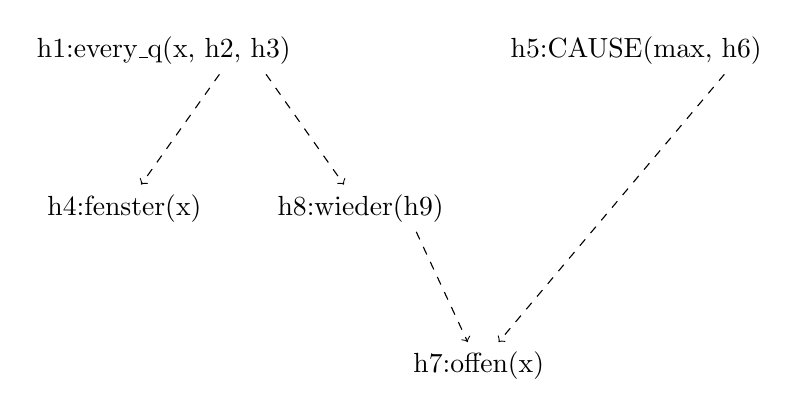
\begin{tikzpicture}
%    \draw (-5,10) to[grid with coordinates] (5,-.5);
    \node(offen)   at (0,0) {h7:offen(x)};
    \node(fenster) at (-4.5,2){h4:fenster(x)};
    \node(every-q) at (-4,4){h1:every\_q(x, h2, h3)};
    \node(wieder)  at (-1.5,2){h8:wieder(h9)};
    \node(cause)   at (2,4) {h5:CAUSE(max, h6)};

    \draw[->,dashed]   (wieder.-23)  to (offen);   
    \draw[->,dashed]   (every-q.-23)  to (fenster);
    \draw[->,dashed]   (every-q.-13)  to (wieder);
    \draw[->,dashed]   (cause.-15)    to (offen);
    \end{tikzpicture}
\caption{Dominanzgraph für \emph{Max alle Fenster wieder öffnete}\label{Abbildung-Max-alle-Fenster-wieder-oeffnete}}
\end{figure}
Um diese Dominanzgraphen aus dem Graphen ohne \emph{wieder} zu erhalten, muss nur der Ausdruck h8:wieder(h9)
eingefügt werden und Dominanzbedingungen, die verlangen, dass $h9$ Quantoren dominiert, die rechts
von \emph{wieder} stehen bzw.\ von Quantoren dominiert wird, die links von \emph{wieder}
stehen. Dafür habe ich 2008 eine Analyse implementiert, die sich die Kodierung der Valenz zu Nutze
macht, die in Kapitel~\ref{sec-realized} vorgestellt wird. Im Zusammenhang mit Kasusvergabe hat
\citet{Meurers99b} so genannte Spirits eingeführt. Damit wird es möglich, den Kasus für \emph{diesen
  Roman} in Abhängigkeit vom finiten Verb zu vergeben.
vom 
\eal
\ex Diesen Roman vorgelesen hat Max gestern.
\ex Dieser Roman vorgelesen wird nur selten.
\zl
Die Kombination von \emph{diesen}/\emph{dieser} \emph{Roman} mit \emph{vorgelesen} ist immer gleich
  und erst bei Kombination mit dem finiten Verb wird entschieden, welchen Kasus die NP am Satzanfang
  haben muss. Genauso verhält es sich mit der Kongruenz:
\eal
\ex Alle Fenster geöffnet hat Max gestern.
\ex Alle Fenster geöffnet werden nur selten.
\zl
Wenn die Nominalphrase innerhalb von \emph{alle Fenster geöffnet} im Nominativ steht, muss das
finite Verb mit ihr kongruieren. In Meurers' Ansatz werden deshalb Argumente, die schon realisiert
wurden, immer noch in den Valenzlisten ihrer Köpfe repräsentiert. Es wird lediglich das binäre
Merkmal \textsc{realized} von $-$ auf $+$ gesetzt. Das bedeutet aber, dass man diese Information
auch für die Beschränkungen von Skopus benutzen kann.
\ea
dass die Busfahrerin wieder alle Fenster öffnet
\z
In dem Moment, in dem \emph{wieder} mit \emph{alle Fenster öffnet} kombiniert wird, ist klar, dass
die NP für das Objekt \emph{alle Fenster} den \textsc{realized}"=Wert $+$ hat und die Subjekts-NP
den \textsc{realized}"=Wert $-$. Das bedeutet, man kann eine Beschränkung festlegen, die sagt, dass
alle NPen, die bei der Kombination bereits realisiert sind, im Skopus von \emph{wieder} sein müssen,
wohingegen alle NPen, die noch nicht realisiert wurden, Skopus über \emph{wieder} haben müssen.

(\mex{1}) zeigt den entsprechenden Lexikoneintrag für \emph{wieder}:
\eas
\label{le-wieder}%
Lexikoneintrag für \emph{wieder}:\\
\avm{
[ cat & [ head & [\type{adv}\\
                  mod & [ cat &  [ head  & verb\\
                                   comps & \ibox{1} ]]\\
                          cont & [ ltop & \ibox{2}\\
                                   ind  & \ibox{3} ]]\\
          spr  & <>\\
          comps & <> ]\\
  cont & [ ltop & \ibox{4}\\
           ind  & \ibox{3}\\        
           rels & < [\type{wieder}\\
                     lbl  & \ibox{4}\\
                     arg1 & \ibox{5}] >\\
           hcons & < [\type{qeq}\\
                      harg & \ibox{5}\\
                      larg & \ibox{2} ] > \+ outscope-realized(\ibox{1}) ] ]
}
\zs
\itdopt{Runde Klammern sind zu groß.}
\emph{wieder} modifiziert ein Verb mit einer \compsl \ibox{1}. \emph{wieder} ist ein Adverb, braucht
also weder eine Spezifikator noch ein Komplement. Der \ltopw von \emph{wieder} ist identisch mit dem
Label der \relation{wieder}"=Relation. \emph{wieder} hat ein \argone, das das modifizierte Verb im
Skopus hat: \ibox{5} \qeq \ibox{2}. Zusätzlich wird an die Liste der Handle"=Constraints eine Liste
angehängt, die das Ergebnis der Anwendung von \emph{outscope-realized} ist. \emph{outscope-realized} wird auf die
\compsl des modifizierten Verbs angewendet \iboxb{1}. Für alle bereits realisierten Quantoren gibt
es eine \qeq-Beschränkung, die auf der linken Seite das Handle von \emph{wieder} \iboxb{5} hat und
auf der rechten Seite das Handle des Quantors des jeweiligen Arguments des modifizierten Verbs. Für
die nicht realisierten Argumente des modifizierten Verbs wird eine Beschränkung in \hcons
aufgenommen, die besagt, dass der Quantor des noch nicht realisierten Arguments \emph{wieder}, also
\ibox{4} dominiert.
\itdopt{
Constraint angeben}
%
% Wie ist das mit dem \argzero von \emph{wieder}? Hat es eins? In ERG gibt es ein event:
%   \ibox{3}. Allerdings gibt es auch bei apparently eins.
%
Interessanterweise funktioniert diese Analyse auch für schwierige Fälle wie (\mex{1}):
\ea 
Alle Fenster öffnen wird Klaus wieder.
%\ex Öffnen wird Klaus alle Fenster wieder.
\z
Obwohl der Allquantor sich innerhalb einer komplexen vorangestellten Phrase befindet, hat
\emph{wieder} Skopus über den Allquantor.

Die entsprechenden Lesarten für Modifikationen durch \emph{wieder} lassen sich also problemlos ohne
leere Elemente für CAUSE und BECOME ableiten. Es wird genauso eine Dekomposition der Wortbedeutung
von \emph{öffnen} vorgenommen, die dekomponierte Bedeutung ist aber einem einzigen Element, dem Verb, zugeordnet. Durch
Unterspezifikation der Skopusverhältnisse im Lexikon lassen sich dann die entsprechenden Lesarten
ableiten.



%\section*{Kontrollfragen}

\questions{
\begin{enumerate}
\item Was versteht man unter Linking?
\item Wie wird in der HPSG eine Verbindung zwischen Form und Bedeutung eines (komplexen)
      sprachlichen Zeichens hergestellt?
\end{enumerate}
}

%\section*{Übungsaufgaben}

\exercises{
\begin{enumerate}
\item Wie kann man den semantischen Beitrag von \emph{lacht} repräsentieren? Geben Sie den
  Lexikoneintrag für \emph{lacht} an und berücksichtigen Sie das Linking.
\item Geben Sie die vollständige Merkmalbeschreibung für die Wortfolge in (\mex{1}), wie sie in
  \emph{dass Aicke lacht} vorkommt, an: 
      \ea
      Aicke lacht
      \z
      Dabei soll sowohl die syntaktische Struktur als auch der Bedeutungsbeitrag berücksichtigt werden.

\item Laden Sie die zu diesem Kapitel gehörende Grammatik von der Grammix"=CD
(siehe Übung~\ref{uebung-grammix-kapitel4} auf Seite~\pageref{uebung-grammix-kapitel4}).
Im Fenster, in dem die Grammatik geladen wird, erscheint zum Schluss eine Liste von Beispielen.
Geben Sie diese Beispiele nach dem Prompt ein und wiederholen Sie die in diesem Kapitel besprochenen
Aspekte. Sie können auch selbst Beispiele aus den Wörtern konstruieren, die Sie in der Datei
\texttt{lexicon.pl} finden. Betrachten Sie die grafischen Repräsentationen der MRSen und lassen Sie sich die
verschiedenen geskopten MRSen anzeigen, wenn die Beispiele MRSen mit mehreren Lesarten haben.
\end{enumerate}
}




\furtherreading{
Die Interpretation semantischer Repräsentationen konnten hier nur knapp angerissen
werden. \citet{Lohnstein2011a} gibt eine ausführlichere Einführung in Aussagenlogik, Prädikatenlogik
und die Interpretation entsprechender Ausdrücke.

\citet{KR2024a} geben einen Überblick über Semantik im Rahmen der HPSG. \citet{DKW2024a}
beschäftigen sich mit Argumentstruktur und Linking.

Der Artikel von
\citet{CFPS2005a} stellt MRS vor. Ich kann mich erinnern, dass ich in den 90ern diesen Artikel nicht
verstehen konnte, obwohl ich an einer Grammatik gearbeitet habe, die eine MRS enthielt. Ich habe
damals gemeinsam mit Walter Kasper an der deutschen \Verbmobil-Grammatik gearbeitet. Das Buch von
\citet{BB2005a} hat mir sehr dabei geholfen, die Grundidee von Semantikframeworks mit
Unterspezifikation zu verstehen. Das Buch kommt mit einer Prolog"=Implementation der entsprechenden
Grammatikfragmente, so dass man Dinge selbst ausprobieren kann. Ich hoffe, dass das hier vorliegende
Kapitel verständlich und einfach genug ist. Wenn das nicht der Fall ist, können vielleicht
\citeauthor{BB2005a} helfen oder der Originalartikel von \citeauthor{CFPS2005a}.

}